\documentclass[11pt,a4paper]{article}
\usepackage[T1]{fontenc}
%\usepackage[latin1]{inputenc}
%\usepackage{amssymb,amsmath,a4wide}
\usepackage[utf8]{inputenc}
\usepackage{amssymb,amsmath}
\usepackage{nicefrac}
\usepackage[pdftex]{graphicx}
\usepackage{ctable}
\usepackage{amsmath}
%\usepackage{threeparttable} %na
%\usepackage{tabu} %na
\usepackage{tabularx}
\usepackage{subfig}
\usepackage{rotating}
\usepackage{longtable}
%\usepackage[table]{xcolor} % clash with floatrow
\usepackage{xcolor} 
\usepackage{floatrow}
\usepackage{threeparttable}
%\usepackage[multiple]{footmisc} %na
\usepackage{bm}
\usepackage{fancybox}
%\usepackage{harvard}
\usepackage{geometry}         % Definir les marges
\geometry{verbose,a4paper,tmargin=1in,bmargin=1in,lmargin=1in,rmargin=1in}
\usepackage{setspace}
%\usepackage{ccaption}
\usepackage[colorlinks=true,citecolor=black, urlcolor=black, linkcolor=black]{hyperref}
\usepackage{url}
\newcommand{\email}[1]{\href{mailto:#1}{\nolinkurl{#1}}}
\usepackage[french, english]{babel}  % Placez ici une liste de langues, la derniere etant la langue principale
\usepackage{lscape}
\usepackage{afterpage}
\usepackage{supertabular}    %na            %  mettre pour les grands tableaux en formant paysage. marche avec \begin{landscape}
% style de la biblio : necessaire pour utiliser BibTex, necessite le deuxieme fichier exemple.bib
\usepackage{caption}
%\usepackage[longnamesfirst]{natbib}
\usepackage{natbib}
\bibliographystyle{elsarticle-harv}
\newcommand{\tqdl}{\textquotedblleft}
\newcommand{\tqdr}{\textquotedblright}
\linespread{1.2}
\begin{document}
\title{Global value chains and the transmission of price shocks			\thanks{The author wish to thank Pavel Diev, Hubert Escaith, Guillaume Gaulier, Yannick Kalantzis, Guy Levy-Rueff and Jean-François Ouvrard, as well as participants at Banque de France seminars}\\
\vspace{1cm}
\normalsize{First draft version}
}
\vspace{1cm}
\date{\today}
\author{
	Hadrien Camatte\thanks{Banque de France. E-mail: \email{hadrien.camatte@banque-france.fr}}
	\and
	Guillaume Daudin\thanks{Université Paris-Dauphine, PSL University, CNRS, 8007, IRD, 260, LEDa, DIAL, 75016, Paris, France. Sciences Po, OFCE, 75007, Paris. Corresponding author. E-mail: \email{guillaume.daudin@dauphine.psl.eu}}
	\and
	Violaine Faubert\thanks{Banque de France. E-mail: \email{violaine.faubert@banque-france.fr}}
	\and
	Antoine Lalliard\thanks{Banque de France. E-mail: \email{antoine.lalliard@banque-france.fr}}
	\and
	Christine Rifflart\thanks{Sciences Po, OFCE. E-mail: \email{christine.rifflart@ofce.sciences-po.fr}}
}
%\vspace*{\fill}
\maketitle
\begin{abstract}
{\small \noindent
TO UPDATE
Firms' participation in global value chains strengthens cross-country linkages via trade in intermediate inputs. 
In this paper, we build on three sectoral world input-output datasets  to assess the role of global input-output linkages in the propagation of exchange rate shocks in the international economy. 
 %à faire: productivity shocks More specifically, we study the role of global input-output linkages in transmitting oil prices shocks across economies.
We examine the increasing integration of the European economies since the adoption of the common currency and investigate whether the shortening of global value chains in the wake of the Great Recession has changed the propagation of global price shocks. We provide evidence that, following an appreciation of the domestic currency, the direct effect of global price shocks, i.e. the effect resulting from the share of imported final and intermediate goods in domestic consumption, explains the bulk of the propagation of global shocks to domestic consumer prices. By contrast, we find a limited role for the additional transmission of lower domestic input prices to other sectors of the domestic economy and other countries occuring during subsequent production cycles. Finally, building on sectoral data, we examine which sectors experience higher spillovers from global price shocks.
%We also contribute to the literature on global input-output linkages by assessing whether results are consistent across the different world input output databases available (WIOD and TiVA).
}

{\small \bigskip \noindent \emph{JEL Classification}\/: C67, E31, F42, F62\\}
{\small \noindent \emph{Keywords}\/: input-output linkages, spillovers, global value chains, cost-push inflation, euro area \\ }
\end{abstract}

\section{Introduction}
Trade liberalization and lower transportation and communication costs facilitates the fragmentation of production beyond national borders.
As a result, firms' participation in global value chains strengthens cross-country linkages via trade in intermediate inputs. 
Because of imported intermediate goods, fluctuations in the prices of imports that are themselves driven by exchange rate movements affect the domestic cost of production and, ultimately, domestic consumer prices. 
As global value chains contribute to explaining the transmission of macroeconomic shocks across countries, a better understanding of trade spillovers has become paramount.  
In this paper, we build on World Input-Output tables (WIOT hereafter) to investigate how production linkages give rise to nominal spillovers. 
We examine the extent to which domestic consumer prices react to changes in imported intermediate and final goods.
We pay particular attention to euro area countries, as the euro area is more involved in global production chains than other large economies, such as the United States and China \citep{ECB2016} and has been less affected by global value chains shortening than other countries in the years following the Great Recession. 
Building on sectoral data from three different World Input-Output tables, we examine which sectors experience higher spillovers from global inflationary shocks.\\
To preview our findings, we find that...\\
The remainder of the paper is organized as follows. Section \ref{sec:lit} briefly describes the related literature. Section \ref{sec:metho} presents the methodology and the data sources.  Section \ref{sec:prixconso} presents the impact of an exchange rate shock on consumer prices.  Section \ref{sec:prixconsosecteur} examines which of the subcomponents of consumer prices experience higher spillovers from global inflationary shocks.
Section \ref{sec:ccl} provides some concluding remarks and avenues for future research.




We improve on the literature on various respects. First, while most of the literature focuses on production prices, we examine the role of input-output linkages in propagating shocks to consumer prices. 
Secondly, we analyze how sectoral inflation reacts to global inflationnary shocks by examining the main components of consumer prices (manufacturing goods, services, food and energy).  We draw on the World Input-Output Database to examine which sectors experience higher spillovers from global inflationary shocks.

Thirdly, we provide evidence that, following an appreciation of the domestic currency, the direct effect of global inflationary shocks, i.e. the contribution of first-round effects on imported final and intermediate goods in domestic consumption, explains the bulk of the propagation of global shocks to domestic prices. By contrast, we find a limited role for the additional transmission of lower domestic input prices to other sectors of the domestic economy and other countries occuring during subsequent production cycles.


GD Interestingly, this limited role is additive rather than multiplicative. It adds from 0.02 to 0.04 to the price elasticity

PEUT-ÊTRE We assess whether results are robust to the use of different databases (WIOD versus OECD-ICIO). 


\label{sec:intro}


\section{Related literature}
\label{sec:lit}

CR : DONNER PLUS D'ÉLEMENTS DANS LE CONTENU DES PAPIERS

A recent literature examines whether trade in intermediate inputs is an important source of inflation synchronization across countries.
\cite{Auer2017} document that the cross-border propagation of cost shocks through input-output
linkages contributes substantially to synchronizing producer price inflation across countries, combining data on sectoral domestic and international input trade from the World Input Output
Database (WIOD) and producer price indices. By contrast, exchange rate movements and the degree of pricing-to-market are found to play no role in synchronizing inflation across countries.
\cite{AntoundeAlmeida2016} show that the cross-border sectors pairs which trade more intensively with each other in intermediate inputs display higher PPI inflation correlation, indicating  price spillovers along the global supply chain.\\

Our research is also related to the literature on exchange rate pass-through, in particular in an environment where intermediate inputs account for a large share of imports. For instance,  \cite{Goldberg2010} show that imported intermediate inputs are the dominant channel through which changes in import prices pass to CPI inflation.\\

\subsection{The Input-Output model applied to a shock on production costs.}
\label{subsec:io}
The widely known Leontief's production model (or I-O model) studies the impact of a demand shock in a domestic economy \citep{Leontief1951}. The trade in value-added analysis reconciles international trade statistics with national I-O tables, and thus allows Leontief's analysis to be extended to an international context. A number of studies \citep{Hummels2001,Daudin2006,Daudin2011, DeBacker2012,Johnson2012,Koopman2014, Amador2015,Los2016} analyze the value added content of world trade. Some authors focus on Asia \citep{Sato2014} or on the euro area \citep{Cappariello2015}.

Leontief's production model has a dual: the price model. Some studies focus on the consequences of a change in production prices based on an I-O model or a SAM (Social Accounting Matrix) model in developing countries. Leontief's price model is broadly used in multi-sector, single-country macroeconomic models, for example, to measure the effect of a change in energy prices \citep{Bournay2015, Sharify2013}. Implicitly, \cite{Bems2015} use it as they focus on competitiveness and compute real effective exchange rates weighted by the value-added trade structure to measure the impact of a demand change in value added on value added prices and final expenditure levels. It is at the center of \cite{Cochard2016}. 
\cite{Cochard2016} is an accounting approach to the effect of costs on prices ("cost-push inflation"). Firms' margins are assumed to be fixed. Prices only adjust to absorb cost changes, production techniques are fixed during successive production cycles and inputs substitution (for instance, between countries producing the same goods) is not accounted for, despite variations in relative price. The limitations of this approach are well known \citep{Folloni1994}. In particular, and although the division of global value chains largely takes place within multinational firms, it assumes a unique pricing system based on market prices and independent of firm strategies. Still, this method provides a measure of the vulnerability of each sector to price or productivity shocks \citep{Acemoglu2012,Carvalho2014}. Hence, though unrealistic, it is useful for identifying which countries and sectors are under pressure to adjust their prices when subject to exogenous cost shocks. For instance, it can show which euro area countries benefit most from an appreciation of the euro or whether adopting the euro has increased interdependence between member countries.



\section{The PIWIM model }
\label{sec:metho}
Based on initial work from the OFCE (Observatoire Français des Conjonctures Économiques) \cite{Cochard2016}, we developed a model named «PIWIM» (Push cost Inflation through World Input-output Matrices). This paper makes extensive use of this model.



\subsection{Defining a price shock in a I-O model}
\label{subsec:ioprice}
To identify which countries are most affected by a price shock through value-added and vertical trade flows in international trade, we need a large structural matrix that integrates input flows between sectors, both within each country and between countries.
This matrix traces the sectoral and geographical origin of inputs. \\
The standard I-O model relies on input-output tables registering transactions of goods and services (domestic or imported) at current prices. The I-O tables describe the sale and purchase relationships between producers and consumers within an economy. Each column describes, for each industry $j$, the intermediate consumption of goods and services from the various sectors.
By extension, a "world" I-O table (WIOT hereafter) describe the sale and purchase relationships between producers and consumers in the whole world, differentiating between sectors in different countries.
The WIOT has, on its diagonal, the country blocks with flows of domestic transactions of intermediate goods and services between industries.
The country blocks outside of the diagonal represent international flows of intermediate goods and services via bilateral sectoral exports and imports. \\
Assuming no inputs substitution between industries or countries (i.e. assuming that technical coefficients are fixed), we can derive a price equation under the assumption of complete cost pass-through.\\
%The rows of the table contain information on the distribution of the output of industries over use categories.
$N$ is equal to the product of the number of countries ($I$) and the number of sectors ($J$). Define $\cal A$ the matrix of technical input coefficient of dimension $(N, N)$, and $Y$ the output vector of dimension $(1, N)$. $Y=(y_1\ldots y_N)$.  \\
Define $y_n=p_n*q_n$, with $p_n$ the price and $q_n$ the quantity of product from country $n$ and normalize quantity such as $q_n=1$. \\
Define $P$ the vector of production prices of dimension $(1, N)$ and $V$ the vector of factor income of dimension $(1, N)$ needed to produce one unit of good in each sector. The price of each good is equal to the cost of producing it: $P=P{\cal A}+V$. \\


Suppose an exogenous input price shock occurs. Firms face a change in their costs, which - by hypothesis - they pass on directly to production prices to keep factor incomes constant.
Define ${{\Delta }^{0}}P$ the shock vector of dimension $(1, N)$ computed as the difference between the original price vector $P^0$ and the new vector $P^1$. Then:
\begin{eqnarray*}
\Delta ^{0}P=P^1-P^0=C, 
\end{eqnarray*}
with $C$ the shock vector of dimension (1,N) that contains the direct effect of the shock on output prices.\\
\\
%Under these conditions, for each industry $i$, the shock can be written as the absolute difference between the initial production price and the new production price invoiced following the shock ("shocked price" hereafter).\\
The price increase is passed on to the country-specific industries that use shocked products as intermediate consumptions. The higher the reliance on shocked inputs, the higher the increase in production prices.\\
In a first step, the direct impact of the shock on each country-specific industry's output prices amounts to $\Delta^{1}P=C{\cal A}$.\\
In a second step, the shock is passed on all country-specific industries using these shocked inputs in their production processes. For $k$ production cycles, the increase in production prices amounts to $\Delta^k P=C{\cal A}^k$.\\
As the technical coefficients are smaller than 1, the effect of the initial shock on input prices eventually wears out.
The overall effect of the shock is equal to the sum of the initial shock and all the increases that occurred during the successive production cycles.
Let us call $S$ the total effect of the shock on prices, a vector $(1, N)$ composed of the elements $s_{ij}$ measuring the total effect of the shock on the output price of sector $j$ in country $i$. We have: 

\begin{eqnarray}
S=C {\left( I+{\cal A}+{\cal A}^2+...+{\cal A}^k+...\right)} =C {\left( I-{\cal A} \right)}^{-1}
\label{eq:eqchocprix} 
\end{eqnarray}


with ${\left( I-{\cal A} \right)}^{-1}$ the inverse of Leontief's matrix.

\subsection{The choice of WIOD}
\label{subsec:data}

The world input-output tables are an extension of the national input-output tables. Input-output tables measure the relationships between the producers of goods and services (including imports) within an economy and the users of these goods and services (including exports). The national tables specify, in line, for each industry, the use of the product as intermediate or final use. In a national table, final use includes exports alongside domestic final uses. Exports are not a final use in world input-output tables. They show by which foreign industry a product was produced, and which foreign industry or final user uses the exports of a given country. For example, world input-output tables enable us to identify how much international trade is associated with the consumption of a particular final product. \\
Aggregating national input-output tables in world input-output tables is challenging for many reasons. For example, national input-output tables vary widely in terms of detail and scope, and are therefore not fully consistent. Furthermore, the availability of year-specific national input-output tables is limited, especially for developing economies. Other issues exists. \\
Two datasets including a time dimension for world intput-output tables are available: (\textit{i}) the World Input Output Database (WIOD) and (\textit{ii}) the OECD-ICIO database TiVA.
\paragraph{The World Input Output Database (WIOD)}
The World Input Output Database (WIOD) contains time series of inter-country input-output tables from 2000 to 2014.  It provides "World Input-Output Tables" that reconcile national input-output tables (or supply-use tables) with bilateral trade statistics derive the final symmetric world input-output table. The WIOD covers 43 countries, of which 28 belongs to the European Union and 15 are other major countries that cover, in total, aroud 85$\%$ of world GDP. They contain annual information for 56 industries, comprising primary, manufacturing goods and services sectors. Therefore, for each year a full country-sector input-output matrix traces the importance of a supplying industry in one country for an industry in another country. The values in WIOTs are expressed in millions of U.S. dollars; market exchange rates were used for currency conversion \citep{Timmer2015}. 

% All transactions values are in basic prices, reflecting all costs borne by the producer. These tables are accompanied by Socio-Economic Accounts which contain country sector panel data on employment (number of workers, compensation and share of labor in high, medium and low skilled occupations), capital stocks, gross output and value added).

Table \ref{tab:wiod} shows the economies included in the WIOD.
 
 
\begin{table}[!h]
\begin{threeparttable}
\centering
\centering
\caption{\small{\textbf{Economies included in the World Input-Output Database}}}
\small
\begin{tabular}{ll}
\hline\hline
Europe & Austria, Belgium, Bulgaria, Croatia, Cyprus, Czech Republic, Denmark,\\
& Estonia, Finland, France, Germany, Greece, Hungary, Ireland, Italy,\\
& Latvia, Lithuania, Luxembourg, Malta, Netherlands, Norway, Poland,\\
&Portugal, Romania, Slovakia, Slovenia, Spain, Sweden, Switzerland,\\
& United Kingdom\\
North  America& Canada, United States\\
Latin America & Brazil, Mexico \\
Asia-Pacific & Australia, China, India, Indonesia, Japan, Korea, Taiwan\\
Other & Russia, Turkey\\
\hline\hline
\end{tabular} 
\label{tab:wiod}
\end{threeparttable}
\end{table} 

\paragraph{The Statistics on Trade in Value Added (TiVA) database}
The TiVA database is compiled by the OECD and the WTO. It builds on the OECD harmonized individual country input-output tables to provide matrices of inter-industrial flows of goods and services in current prices (USD million).
We use two versions of this database. The third revision, from 2016, includes for 64 economies (i.e. 35 OECD Countries, 28 non-OECD economies and the Rest of the world) and 34 industries, and covers the every year between 1995 and 2011.
The fourth revision, from 2018, includes one more economy (Kazakhstan) and 36 sectors and covers every year between 2005 and 2015.
Beside coverage, there are extensive differences between both TiVA databases (\cite{OECD2018}).
Table \ref{tab:tiva} shows the economies included in the TiVA databases.

\begin{table}[!h]
\begin{threeparttable}
\centering
\centering
\caption{\small{\textbf{Economies included in the TiVA databases}}}
\small
\begin{tabular}{ll}
\hline\hline
Europe & Austria, Belgium, Bulgaria, Croatia, Cyprus, Czech Republic, Denmark,\\
& Estonia, Finland, France, Germany, Greece, Hungary, Iceland, Ireland, Italy,\\
& Latvia, Lithuania, Luxembourg, Malta, Netherlands, Norway, Poland,\\
&Portugal, Romania, Slovakia, Slovenia, Spain, Sweden, Switzerland,\\
& United Kingdom\\
North  America& Canada, United States\\
Latin America & Argentina, Brazil, Chile, Colombia, Costa Rica, \\ 
&Mexico (differentiating between three (Rev3) or two (Rev4) Mexico), Peru\\
Asia-Pacific & Australia, Cambodia, China (differentiating between four (Rev3) or three (Rev4) China), \\
& Hong Kong SAR, India, Indonesia, Japan, Khazakhstan (in Rev4), Korea, Malaysia, \\
& New Zealand, Philippines, Singapore, Taiwan, Thailand, Viet Nam\\
Other & Brunei, Israel, Morocco, Russia, Saudi Arabia, South Africa, Tunisia, Turkey\\
\hline\hline
\end{tabular} 
\label{tab:tiva}
\end{threeparttable}
\end{table} 


\paragraph{Major differences between the WIOD and TiVA databases}
The WIOD and TiVA databases have a number of distinguishing characteristics (see \cite{Timmer2015} for details). The most relevant difference for our analysis relates to the treatment of imports by use category. National input-output statistics provide the use of products by industries and final consumers, but the country of origin of products is unknown. Therefore, one has to breakdown product import statistics by category of use in the construction of world input-output tables.\\
The TiVA database relies on the so-called "import proportionality assumption". The domestic input-output tables show transactions between domestic industries. As a complement to these tables, supplementary tables break down total imports by user (industry and the different categories of final demand). Some countries provide these import tables in conjunction with their input-output tables, but in other cases they are derived by the OECD. Mexico and China benefit from a special treatment, but for the other countries the main assumption used is that the share of imports in any product consumed directly as intermediate consumption or final demand (except exports) is the same for all end-uses (the "proportionality assumption") \footnote{See \cite{OECD2011} for details.}.\\
Various studies have found that this assumption can be misleading, as import shares vary significantly across end-uses. \cite{Feenstra2012} find that shares of imported materials may differ substantially across U.S. industries. Based on Asian input-output tables, \cite{Puzzello2012} finds that the proportionality assumption understates the use of foreign intermediate inputs. It is likely to be particularly binding for developing countries, as the import content of exports is usually higher than the import content of products used for domestic consumption.\\
To address this issue, the WIOD database uses bilateral trade statistics to derive import shares for three end-use categories (intermediate use, final consumption and investment) by mapping detailed six-digit products international trade statistics based on product descriptions \citep{Dietzenbacher2013}.\\
To sum up, the WIOD includes information on bilateral industry-specific input use, whereas such information exists only in imputed form in TiVA. Therefore, we focus on the WIOD database in our analysis \footnote{Results obtained with the 2016 and 2018 TiVA databases are available upon request.}. 


\subsection{Nominal exchange rate shock}
\label{subsec:chocchange}

We implement an exchange rate shock using the WIOD databases described above. 
The appreciation of a currency against other currencies leads, for the shock-stricken country, to a fall in the domestic-currency price of its imports and an increase in the foreign-currency price of its exports. We focus on the disinflationary impact of this shock on the shock-stricken country though we also estimate, conversely, its inflationary impact on countries that directly and indirectly consume, through third countries linkages, inputs from the shock-stricken country.\\
However, this shock cannot be analyzed applying the method described in \ref{subsec:ioprice} because the value of the price, besides depending of the nationality of the input-providing sector, also depends on the nationality of the input-using sector.  Suppose a world with two countries A and B, each having its own national currency, and a currency for international transactions, the dollar.
Assuming a 100$\%$ appreciation of the currency of country $A$ against the other two currencies, the production prices of country $A$ expressed in dollars would double compared to those of country $B$ expressed in dollars. Country $B$ pays more for its imports of inputs, in dollars as well as in national currency, since the exchange rate of the currency of Country $B$ against the dollar has not changed. Conversely, the imported input prices in country $A$ remain constant in dollar terms, since production prices of country $B$ have not changed and fall by half once expressed in national currency.\\
We assume that producers have no margin behavior and pass through the exchange rate shock fully on to their production prices. The change in the prices of imported goods is therefore transmitted to all domestic prices, both directly and through inter-industry linkages. These upward (downward) movements for country $B$ (country $A$) affect all input prices in each of the countries.\\
The effects of the shock spread over multiple production cycles. At the end of this process, the overall impact of the shock in dollar terms is equal, for the shocked country $A$, to the rise in production prices due to the exchange rate shock, minus direct and indirect decreases (via interindustry linkages in the country), in national currency and then converted back into dollar terms, in the prices of inputs imported from $B$ and disseminated to all branches. The overall impact on production prices in dollar terms in country $A$ is therefore lower than the initial exchange rate shock. For country $B$, the final impact is to the cumulative direct and indirect effects of higher prices of inputs imported from country $A$ and disseminated to all industries.\\

In a global economy composed of $I$ countries, each with $J$ sectors, the appreciation of a country's currency $i$ against all other currencies translates into a rise in country $i$'s prices in dollars. The production price of each sector will vary in dollar terms by: $c_\$^i$ in the shock-stricken country$~i$ and 0 in other countries. \\
Hence, for each sector $j$ in country  $i$:
\begin{eqnarray*}
 {{\Delta }^{0}}p_{\${ij}}=p_{\${ij}}^{1}-p_{\${ij}}^{0}=c_{\${ij}}=c_{\$}^i
  \end{eqnarray*}	
And for each sector $j$ in country $k (k\ne i)$,
\begin{eqnarray*}
 {{\Delta }^{0}}p_{\${kj}}=p_{\${kj}}^{1}-p_{\${kj}}^{0}=c_{\${kj}}=0
 \end{eqnarray*}	
To simplify, initial output prices for each sector are normalized to 1 and exchange rates to 1:1. A 100$\%$ appreciation in the exchange rate of a currency against other currencies therefore corresponds to an absolute shock of +1, with production prices in the shock-stricken country rising from 1 to 2 dollars.\\
The appreciation affects producers through changes in relative prices between countries and, therefore, through changes in input prices traded between the shock-stricken country $i$ and other countries. \\
Consider first the direct impact (in absolute terms) on other countries of the rise in imported input prices from shocked country $i$. For any sector l of a country $k$ $(k\ne i)$, the increase in the producer price depends directly on the quantity of inputs imported from the shock-stricken country $i$, weighted by the variation in level of the price of inputs in dollars (i. e. the exchange rate shock):\\
\begin{eqnarray}
\Delta ^1 p_{\${kl}}=c_\$^i*a_{kl,i1}+\ldots+c_\$^i.a_{kl,ij}+\ldots+c_\$^i.a_{kl,iJ}=\underset{j=1}{\overset{J}{\mathop\sum}}\,c_\$^i.a_{kl,ij}=c_\$^i.\underset{j=1}{\overset{J}{\mathop\sum}}\,a_{kl,ij}  
\label{eq:eq1} 
\end{eqnarray}
With $a_{kl,ij}$ the quantity of inputs from the country $i$'s sector $j$ needed to develop a production unit for the country's $k$ sector $l$. \\
For the shocked country, the shock has a disinflationary effect on domestic production prices. In national currency, the production prices of imported inputs fall in each sector by $c^i=-\frac{c_\$^i}{1+{c_\$^i}}$, or by 0.5 with $c_\$^i=1$. \\
This decline then spreads to all domestic-input using sectors. In sector $j$ of the shocked country $i$, this fall amounts in national currency to: \\
\begin{eqnarray*}
\Delta^1p_{ij}=\underset{l=1}{\overset{l=J}{\mathop \sum}}\,c^i.a_{ij,1l}+\ldots +\underset{l=1}{\overset{{l}=J}{\mathop \sum }}\,c^i.a_{ij,kl}+\underset{l=1}{\overset{l={J}}{\mathop \sum }}\,c^i.{{a}_{ij,pl}}=\left( -\frac{c_\$^i}{1+c_\$^i}\right).\underset{\begin{matrix}k=1\\k\neq i\\\end{matrix}}{\overset{k=I}{\mathop\sum}}\,\left[\underset{l=1}{\overset{l=J}{\mathop\sum}}\,a_{ij,kl}\right] 
\end{eqnarray*}
This level shock can be converted into dollars: \\
\begin{eqnarray}
{{\Delta }^{1}}{{{p}}_{\$ij}}=\left(1+c_\$^i\right).\left(-\frac{c_\$^i}{1+c_\$^i}\right)\underset{\begin{matrix}k=1\\k\neq i\\\end{matrix}}{\overset{{k}={I}}{\mathop\sum}}\,\left[\underset{\text{l}=1}{\overset{{l}={J}}{\mathop\sum}}\,{{{a}}_{ij,kl}}\right] 
\label{eq:eq2}
\end{eqnarray}
We therefore know the direct impact of the shock on all input prices of all countries.
In matrix notation, we create two matrices that build on the world input-output matrix $A$ defined in \ref{subsec:ioprice}. These two matrices retain only the direct effects of the exchange rate shock on the price of goods imported by the shocked country $i$ and the direct effects of the exchange rate shock on the price of goods imported by the rest of the world from the shocked country $i$. To formalize the initial impact of the shock on the price of traded goods, we neutralize the impact of an input price shock on the price of domestic inputs as well as on the price of inputs traded between countries that are not shocked.\\
Let us first look at the shock from the perspective of countries that import inputs from country $i$.\\
Let $C_\$^i$ be the vector of change in production prices in dollars following the 
%{100$\%$}
appreciation of the currency of country $i~$ against all other currencies.
%, corresponding to an absolute shock of $+1$ dollar for all sectors in country $i$. \\
Hence,
\begin{eqnarray*}
C_\$^i=\left(0\ldots0\ldots c_{\$ij}\ldots c_{\$ik}\dots 0\ldots0\right)
\end{eqnarray*}
with $c_{\$ij}=c_{\$ik}=c_\$^i
%=1
$
for all sectors $j$ and $k$ in the shocked country $i$.\\
Building on Equation \ref{eq:eq1}, we write the direct impact of the exchange rate shock on the other countries as the product of the shock vector $C_\$^i$ and a matrix ${\cal B}$. ${\cal B}$ builds on the large matrix ${\cal A}$ of technical coefficients, but only keeps the coefficients of each country's sectoral inputs imported from the shocked country $i$. The other coefficients are replaced by 0, including those of the block of country $i$ concerning the domestic inputs of the shocked country $i$. The direct impact of the appreciation of a currency against the dollar on the price of inputs in countries that are not shocked is equal to $C_\$^i{\cal B}$ with
\begin{eqnarray}
C_\$^i{\cal B}=\left(0\ldots c_\$^i \ldots 0\right)\left(\begin{matrix}0&\cdots&0\\a_{11,ij}&0&a_{IJ,ij}\\0&\cdots&0\\\end{matrix}\right) 	
\label{eq:eq3}
\end{eqnarray}
where each $a_{kl,ij}$ element of the line block represents the technical coefficient related to imports of inputs by sector $l$ in country $k$ (with $k\ne i$) from sector $j$ of country $i$.\\
Let us now consider the shock from the perspective of the shocked country $i$.\\
\\

%\textcolor {blue}{GD Je ne comprends pas. La valeur en dollar des inputs importés par le pays choqué ne devrait pas varier ? C'est leur valeur en monnaie nationale qui change ?}
%Define ${{\tilde{C}}_{\$}}$ the vector of change in input prices imported by country i, in dollars, $( -c_{\$i}\ldots0\ldots-c_{\$i})$. 
%
%From Equation \ref{eq:eq2}, we can write the direct impact for country $i$ of the fall in input prices from the rest of the world. The direct impact corresponds to the product of the shock vector ${\tilde{c}}$  and a matrix ${\tilde{B}}$. ${\tilde{B}}$ builds on the large matrix A of which only the country blocks of the inputs imported by country $i$ from other countries have been retained. The other coefficients are replaced by 0, including those of the block of country $i$ concerning the domestic inputs of the shocked country $i$. \\
%
%The direct impact of the appreciation of the shocked country $i$ on the price of its inputs corresponds, in dollars, to ${{\tilde{c}}_{\$}}{\tilde{B}}$ with: 
%\begin{eqnarray}
%{{\tilde{c}}_{\$}}{\tilde{B}}=\left(-{{{c}}_{\$i}}\ldots0\ldots-{{{c}}_{\$i}}\right)\left(\begin{matrix}0&\ldots{{{a}}_{{i}1,11}}\ldots&0\\0&0&0\\0&\ldots{{a}_{\text{il,pn}}}\ldots&0\\\end{matrix}\right) 
%\label{eq:eq4}
% \end{eqnarray}
%where each ${{{a}}_{{ij,kl}}}$ element in the column block represents imports of inputs by sector $j$ in country $i~$from sector$~l$ in country $k$.
%
%\textcolor {blue}{GD Je suis dans la perplexité. Proposition de changement}

Define $C^i$ the vector of change in production prices everywhere expressed in country $i$'s currency, 
$\left(-\frac{c_\$^i}{1+c_\$^i},\ldots0\ldots,-\frac{c_\$^i}{1+c_\$^i} \right)$. \\

From Equation \ref{eq:eq2}, we can write the direct impact for country $i$ of the fall in input prices from the rest of the world. The direct impact corresponds to the product of the shock vector $C^i$  and a matrix ${\tilde{{\cal B}}}$. ${\tilde{{\cal B}}}$ builds on the large matrix ${\cal A}$ of which only the country blocks of the inputs imported by country $i$ from other countries have been retained. The other coefficients are replaced by 0, including those of the block of country $i$ concerning the domestic inputs of the shocked country $i$. \\

The direct impact of the appreciation of the shocked country $i$ on the price of its inputs corresponds, in national currency, to $C^i{\tilde{{\cal B}}}$ with: 
\begin{eqnarray}
C^i{\tilde{{\cal B}}}=\left(-\frac{c_\$^i}{1+c_\$^i},\ldots0\ldots,-\frac{c_\$^i}{1+c_\$^i} \right)\left(\begin{matrix}0&\ldots{{{a}}_{ij,11}}\ldots&0\\0&0&0\\0&\ldots{{a}_{{ij,IJ}}}\ldots&0\\\end{matrix}\right) 
\label{eq:eq4}
 \end{eqnarray}
where each ${{{a}}_{{ij,kl}}}$ element in the column block represents imports of inputs by sector $j$ in country $i~$from sector$~l$ of country $k$.
We can then convert this direct impact in dollars, by multiplying it by the new value of the national currency in dollars, $\left(1+c_\$^i\right)$. The direct impact of the appreciation of the shocked country $i$ on the price of its inputs corresponds, in dollars, to ${\tilde{C}_\$^i}{\tilde{{\cal B}}}$ with: 
\begin{eqnarray}
{\tilde{C}_\$^i}{\tilde{{\cal B}}}=\left(1+c_\$^i\right).C^i{\tilde{{\cal B}}}=
\left(-c_\$^i\ldots0\ldots-c_\$^i\right)\left(\begin{matrix}0&\ldots{{{a}}_{ij,11}}\ldots&0\\0&0&0\\0&\ldots{{a}_{{ij,IJ}}}\ldots&0\\\end{matrix}\right) 
\label{eq:eq4}
 \end{eqnarray}



%\textcolor{blue}{GD retour au texte}




The direct effect on the world is therefore the sum of these vectors from equations  \ref{eq:eq3} and \ref{eq:eq4}, i. e. $C_\$^i.{\cal B}+{\tilde{C}_\$^i}{\tilde{{\cal B}}}.~$\\
An input price shock then spreads to all sectors in all countries via the global intersectoral exchanges transcribed by the matrix of technical coefficients of the large matrix {\cal A}. This process will be repeated several times, until the effects are completely exhausted.
In the end, the total sectoral effect of the dollar shock is equal to the sectoral shock itself, incremented by changes in input prices due to changes in imported input prices, and by all marginal changes in output prices during the production processes, i. e.:\\
\begin{eqnarray*}
S_\$^i=\Delta{{P}_{\$}^i}=C_\$^i+ \left(C_\$^i.{\cal B}+{\tilde{C}_\$^i}{\tilde{{\cal B}}}\right)+ \left(C_\$^i.{\cal B}+{\tilde{C}_\$^i}{\tilde{{\cal B}}}\right){{\cal A}}+\left(C_\$^i.{\cal B}+{\tilde{C}_\$^i}{\tilde{{\cal B}}}\right){{\cal A}^{2}}+\ldots+\left(C_\$^i.{\cal B}+{\tilde{C}_\$^i}{\tilde{{\cal B}}}\right){\cal A}^k +\ldots \\
\end{eqnarray*}

GD J'AI MODIFIÉ À PARTIR D'ICI
 
 \begin{eqnarray}
S_\$^i=C_\$^i+\left(C_\$^i.{\cal B}+{\tilde{C}_\$^i}{\tilde{{\cal B}}}\right)*{{(I-{\cal A})}^{-1}}	
\label{eq:eqinternationalcurrency}
 \end{eqnarray}
With $S_\$^i$ the total impact vector composed of the elements ${{{s}}^i_{\$kj}}$ showing the total impact of the shock in the exchange rate of country $i$ on country $k$'s sector $j$. Equation \ref{eq:eqinternationalcurrency} gives the absolute evolution of sectoral prices in international currency. The study of this vector is the main objet of \cite{Cochard2016}. //

In contrast, this paper focuses on the internal effect of an exchange rate shock. To obtain the absolute evolution of the sectoral prices of the shocked country in national currency, we remove the exchange rate shock in international currency, multiply the balance by the scalar of conversion equal to $\frac{1}{1+c_\$^i}$ and add the initial exchange rate shock in national currency.

\begin{equation}
\begin{aligned}
	S^i&=C^i  + \left( \frac{1}{1+{{c}_\$^i}}\right)*\left({S_\$^i}-{{C}_{\$}^i}\right)\\
	&=C^i + \left( \frac{1}{1+{{c}_\$^i}}\right)*\left(C_\$^i.{\cal B}+{\tilde{C}_\$^i}{\tilde{{\cal B}}}\right)*{{(I-{\cal A})}^{-1}} 	\\
	&=C^i	+ \left(\hat{C}^i_\$.{\cal B}+{C^i}{\tilde{{\cal B}}}\right)*{{(I-{\cal A})}^{-1}}	
\label{eq:eqdomcurrency}
\end{aligned}
\end{equation}
Where $\hat{C}^i_\$=\left(0 \ldots \frac{c_\$^i}{1+c_\$^i},\ldots 0 \right)$ is the increase in dollar prices of goods from country $i$ used as inputs in all other countries.\\ 
$S^i$ represents the overall impact of a shock on prices in each sector of each country expressed in the shocked currency.
It is quite different from $S$ defined in eq. \eqref{eq:eqchocprix}, because in the case of $S$, the price shock affects all users, whereas in the case of $S^i$, the price shock affects only users that do not share a currency with country $i$. To illustrate the difference, the two country, one sector case is explored in Appendix 1.

To transform this vector in a price level shock in country $i$, $\bar{s}^i$, we need to compute a weighted average of the sectoral effects of the shock. This paper focuses on the price of household consumption. Let $HC^i$ be the vector of sectoral shares in country $i$'s consumption :
\begin{eqnarray*}
HC^i=\left( 
	\begin{array}{c}
	\frac{{hc}_{11}^i}{hc^i} \\
	...\\
	\frac{{hc}_{kj}^i}{hc^i}\\
	...\\
	\frac{{hc}_{IJ}^i}{hc^i}
	 \end{array}
	 \right)
\end{eqnarray*}

Where ${hc}_{kj}^i$ corresponds to household consumption in country $i$ of goods produced by sector $j$ from country $k$ and $hc^i$ represents the total household consumption of country $i$. \\
%For each country, we compute a weighted average of the shock effects, based on three types of aggregation: the sectoral structure of output, the sectoral structure of exports and the sectoral structure of household consumption.\\
%Hence 
%\begin{eqnarray*}
%\overline{s_{i}^{Y}}=\underset{j=1}{\overset{n}{\mathop \sum }}\,\frac{{{s}_{ij}}.{{y}_{ij}}}{{{y}_{i}}}
 %\end{eqnarray*}
%represents the average effect of the shock on output prices in country$~i$, with ${{{s}}_{{ij}}}$ the impact of the shock on the output prices of industry $j$ for country $i$, ${{{y}}_{{ij}}}$ the output of industry $j~$in country $i$ and ${{{y}}_{{i}}}$ the total output of country $i$. \\
%This weighting scheme provides the impact of the shock on each country's production costs ("production prices" hereafter).\\
%The second type of aggregation relies on the sectoral structure of exports. $\overline{s_{i}^{X}}$ provides the average impact of the shock on the export price competitiveness of country $i$. This export price indicator will be referred to as "export price" hereafter. \\
% \begin{eqnarray*}
%\overline{s_{i}^{X}}=\underset{j=1}{\overset{n}{\mathop \sum }}\,\frac{{{s}_{ij}}.{{x}_{ij}}}{{{x}_{i}}},
% \end{eqnarray*} 
%with $x_{ij}$the exports of industry $j$ in country $i$ and $x_{i}$ the total exports of country $i$. \\
%The last type of aggregation relies on the sectoral structure of household consumption.
$\overline{s_{i}}^{i,HC}$ provides the average impact of the shock on the consumer price of country $i$. 
 \begin{eqnarray}
\overline{s}_{i}^{i,HC}=S^i.HC^i=\underset{\begin{subarray}{c}j=1\dots J \\ k=1 \dots I \end{subarray}}{\mathop \sum}\,{{s}_{kj}^i}.\frac{{hc}_{kj}^i}{hc^i}
\label{eq:eq6}
 \end{eqnarray} 
with ${s}_{kj}^i$ is a coefficient of $S^i$ for country $i$. 

\section{The impact of exchange rates fluctuations on consumer prices}
\label{sec:prixconso}
\subsection{Baseline results}
We use the model presented in \ref{subsec:chocchange} to study the absolute value of $\overline{s_{i}}^{i,HC}$ following a 100\% appreciation of the domestic currency versus all other currencies. When the domestic currency appreciates, domestic prices expressed in domestic currency decrease, as imported inputs and imported consumer goods are cheaper. As our model is linear, the exact value of the shock does not matter: choosing 100\% allows us to interpret  $\overline{s_{i}}^{i,HC}$ as an elasticity. As an illustration, using the WIOD database, we find that $\overline{s_{i}}^{i,HC}$ is equal to $-0.055$ for the USA in 2011, meaning that a 100\% appreciation of the dollar would reduce consumer prices by 5.5\%. The following figures report the absolute value of this number ($0.055$).

Additionaly, for Euro area members, we distinguish between the effect of the appreciation of the euro and the effect of the appreciation of a hypothetical national currency. For example, in the case of France, using WIOD in 2011, a 100\% appreciation of the euro would lead to a reduction of domestic prices of 7.6\%. A 100\% appreciation of the hypothetical French national currency would lead a reduction of domestic prices of 12.2\%. 

Figure \ref{fig:comp_WIOD_TIVA}, shows that, despite their differences, using WIOD or TIVA yields very similar results for consumer prices.

\begin{figure}[!h]
\centering
\caption{\footnotesize{\textbf{Comparing consumer price elasticity to an exchange rate appreciation for WIOD, TIVA and TIVA rev4, 2011 and 2014}}}
\begin{tabular}{c}
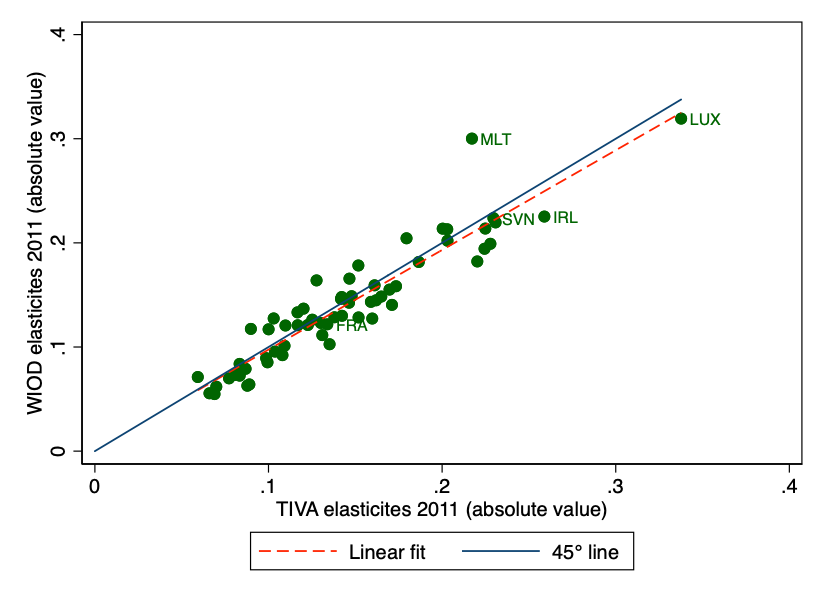
\includegraphics[width=3in, height=2in]{Comparaison_WIOD_TIVA_2011.png}
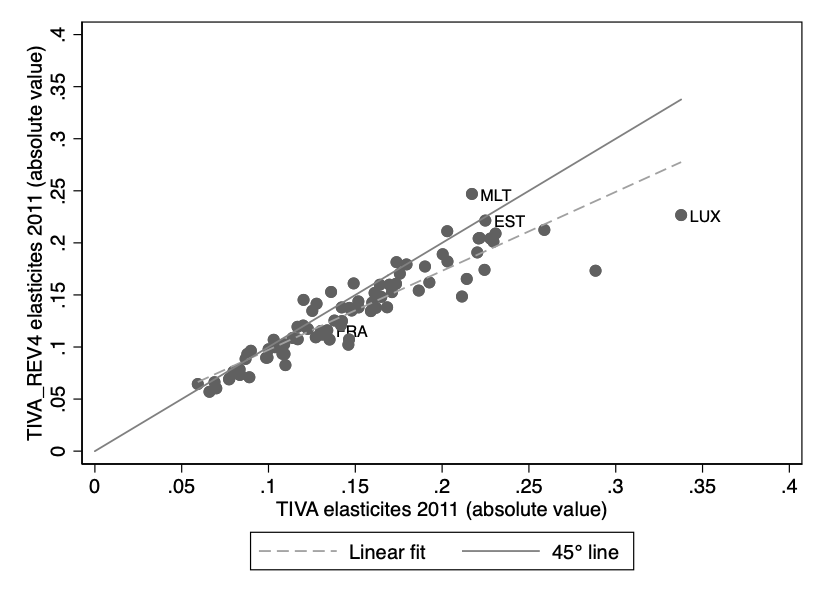
\includegraphics[width=3in, height=2in]{Comparaison_TIVA_REV4_TIVA_2011.png}\\
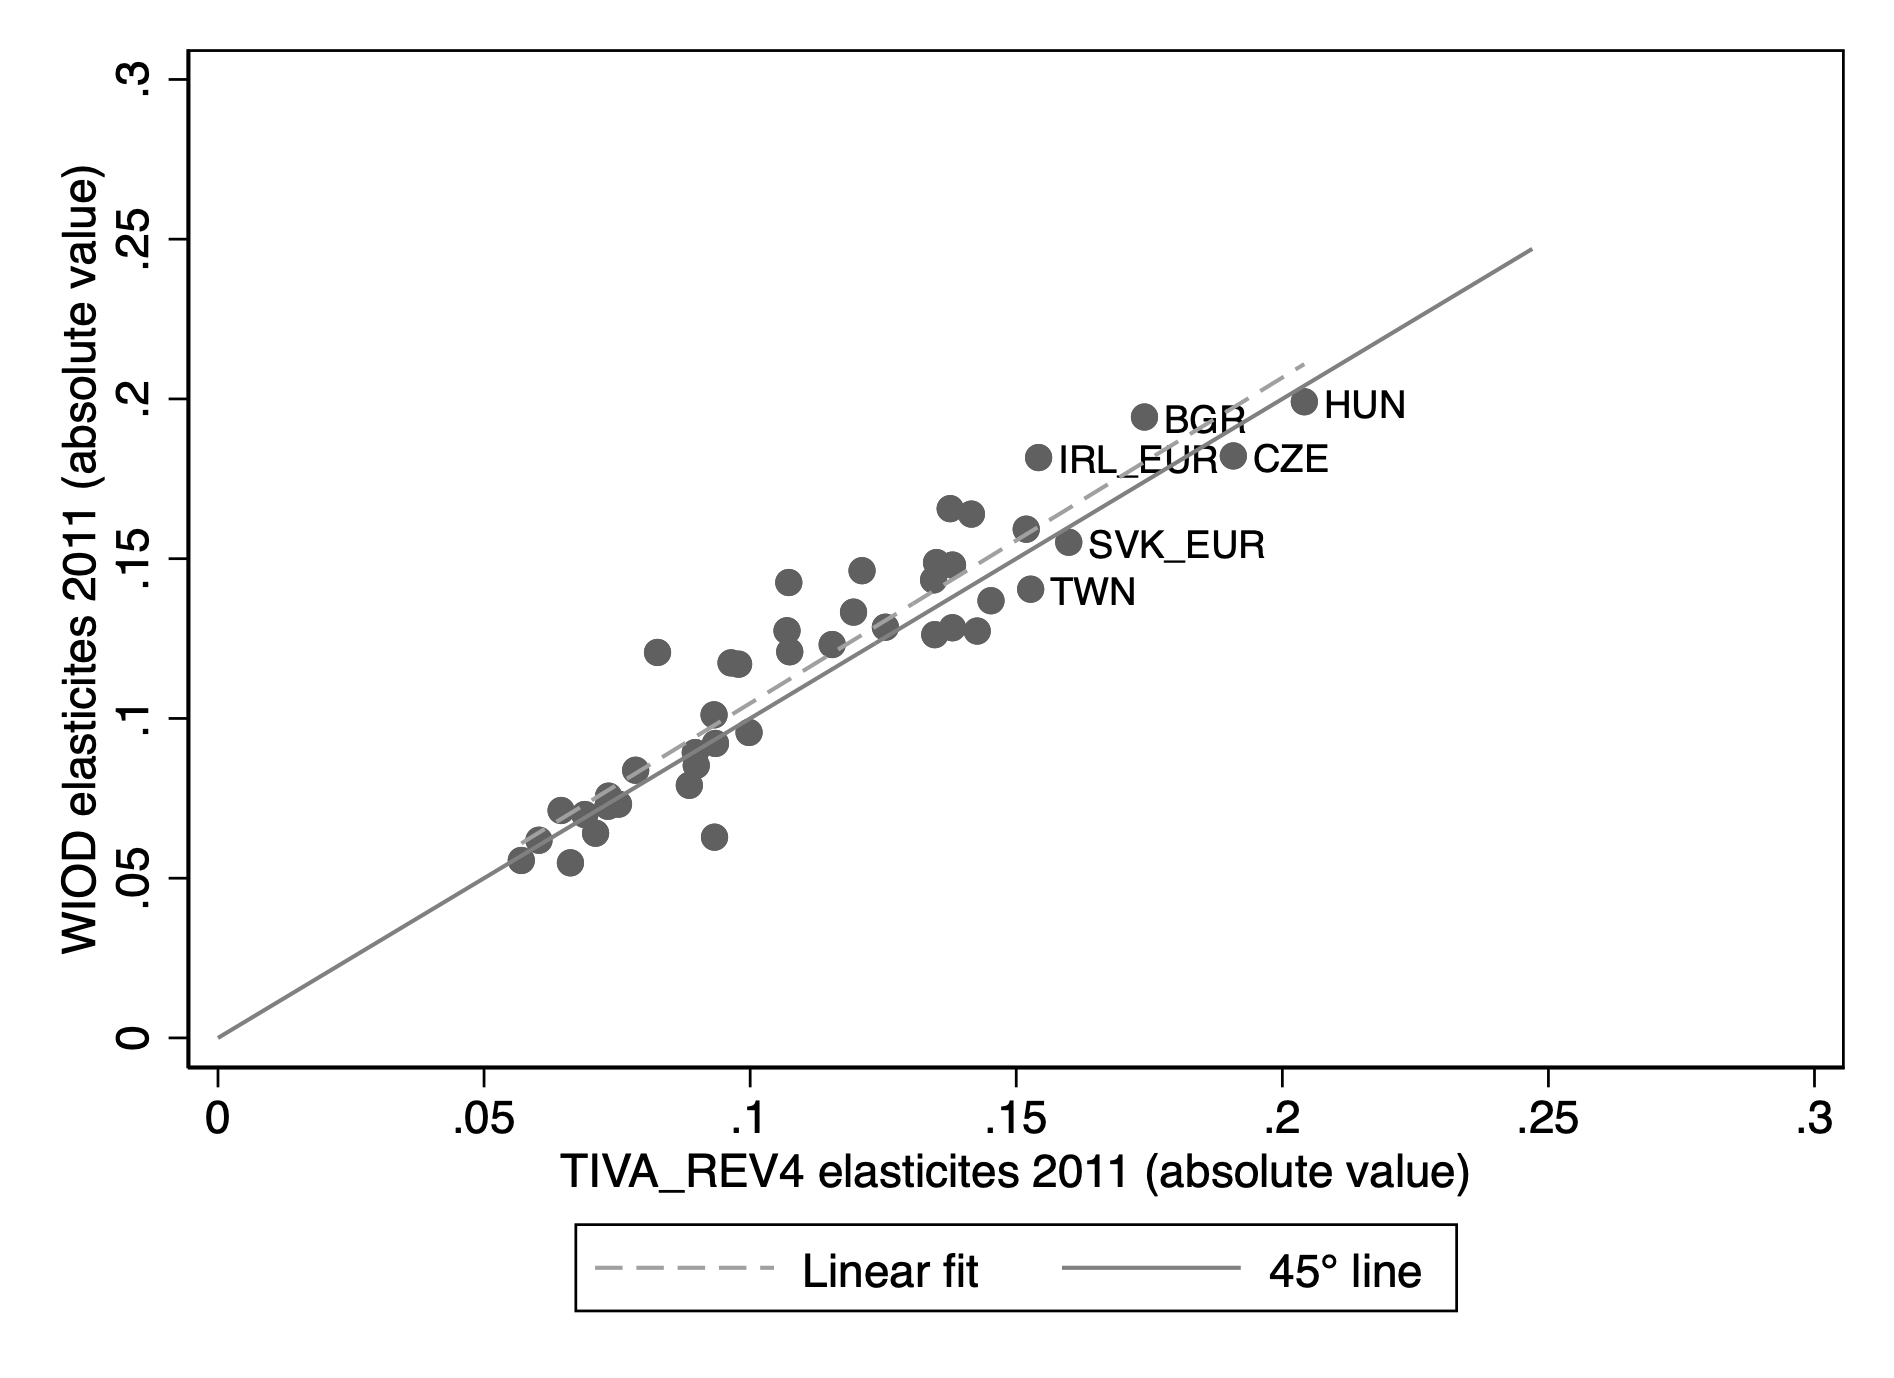
\includegraphics[width=3in, height=2in]{Comparaison_WIOD_TIVA_REV4_2011.png}
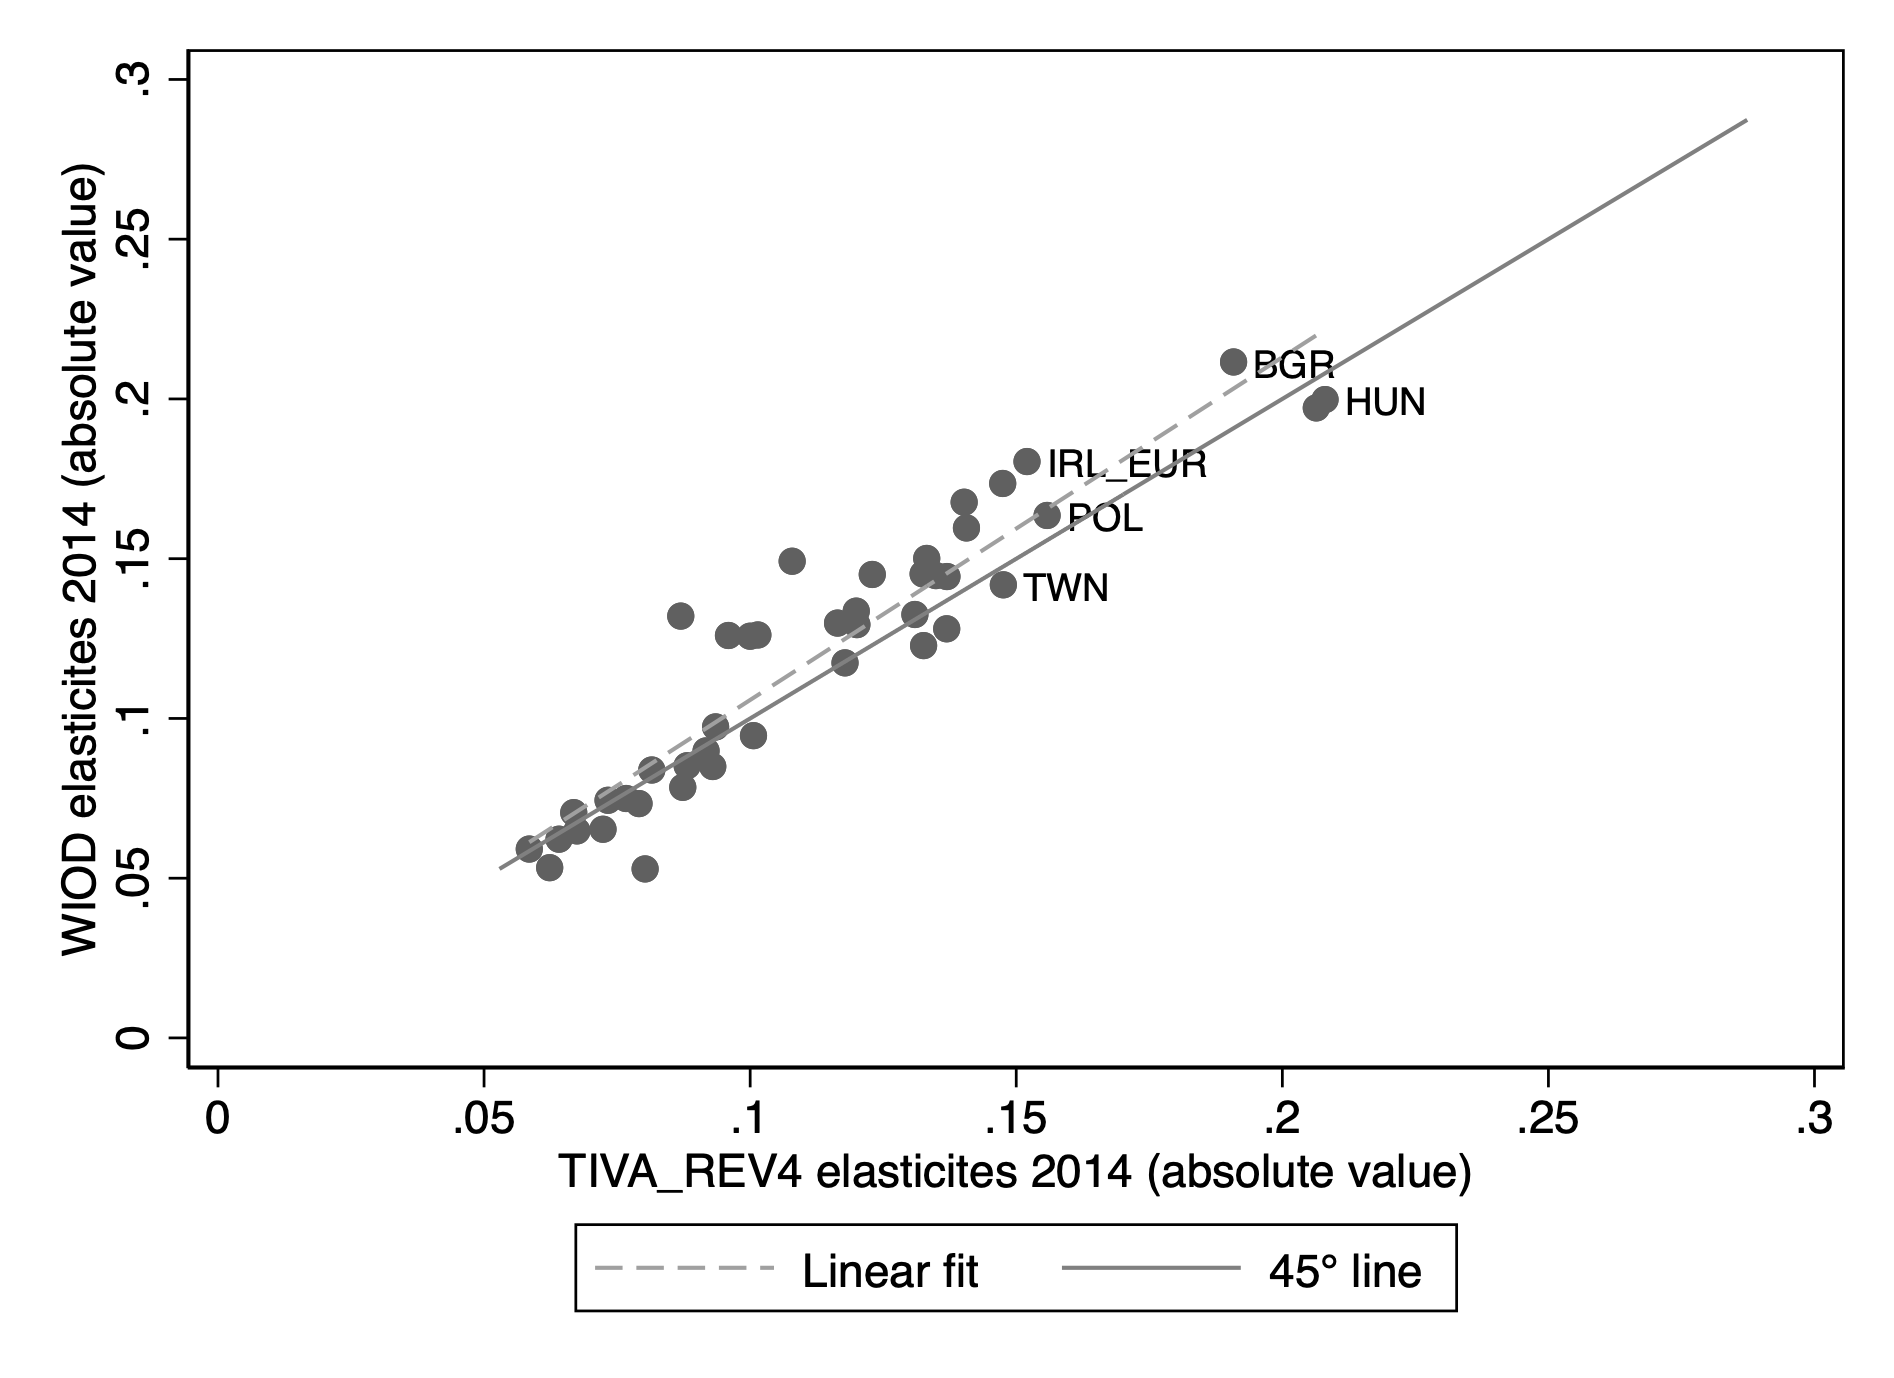
\includegraphics[width=3in, height=2in]{Comparaison_WIOD_TIVA_REV4_2014.png}\\
\floatfoot{Source: WIOD, TIVA rev3 and TIVA rev4}.
\end{tabular}
\label{fig:comp_WIOD_TIVA}
\end{figure}


The evolution of consumer prices elasticity through time is very similar in both source, even if the small difference shown in Figure \ref{fig:comp_WIOD_TIVA} are enough for the mean value of the elasticity of consumer prices to be slightly different depending on the source (see Figure \ref{fig:PIWIM_LONGITUDINAL}).

\begin{figure}[!h]
	\centering
	\caption{\footnotesize{\textbf{Comparing mean consumer price elasticity to an exchange rate appreciation for WIOD and TIVA, 1995-2014}}}
	\begin{tabular}{c}
		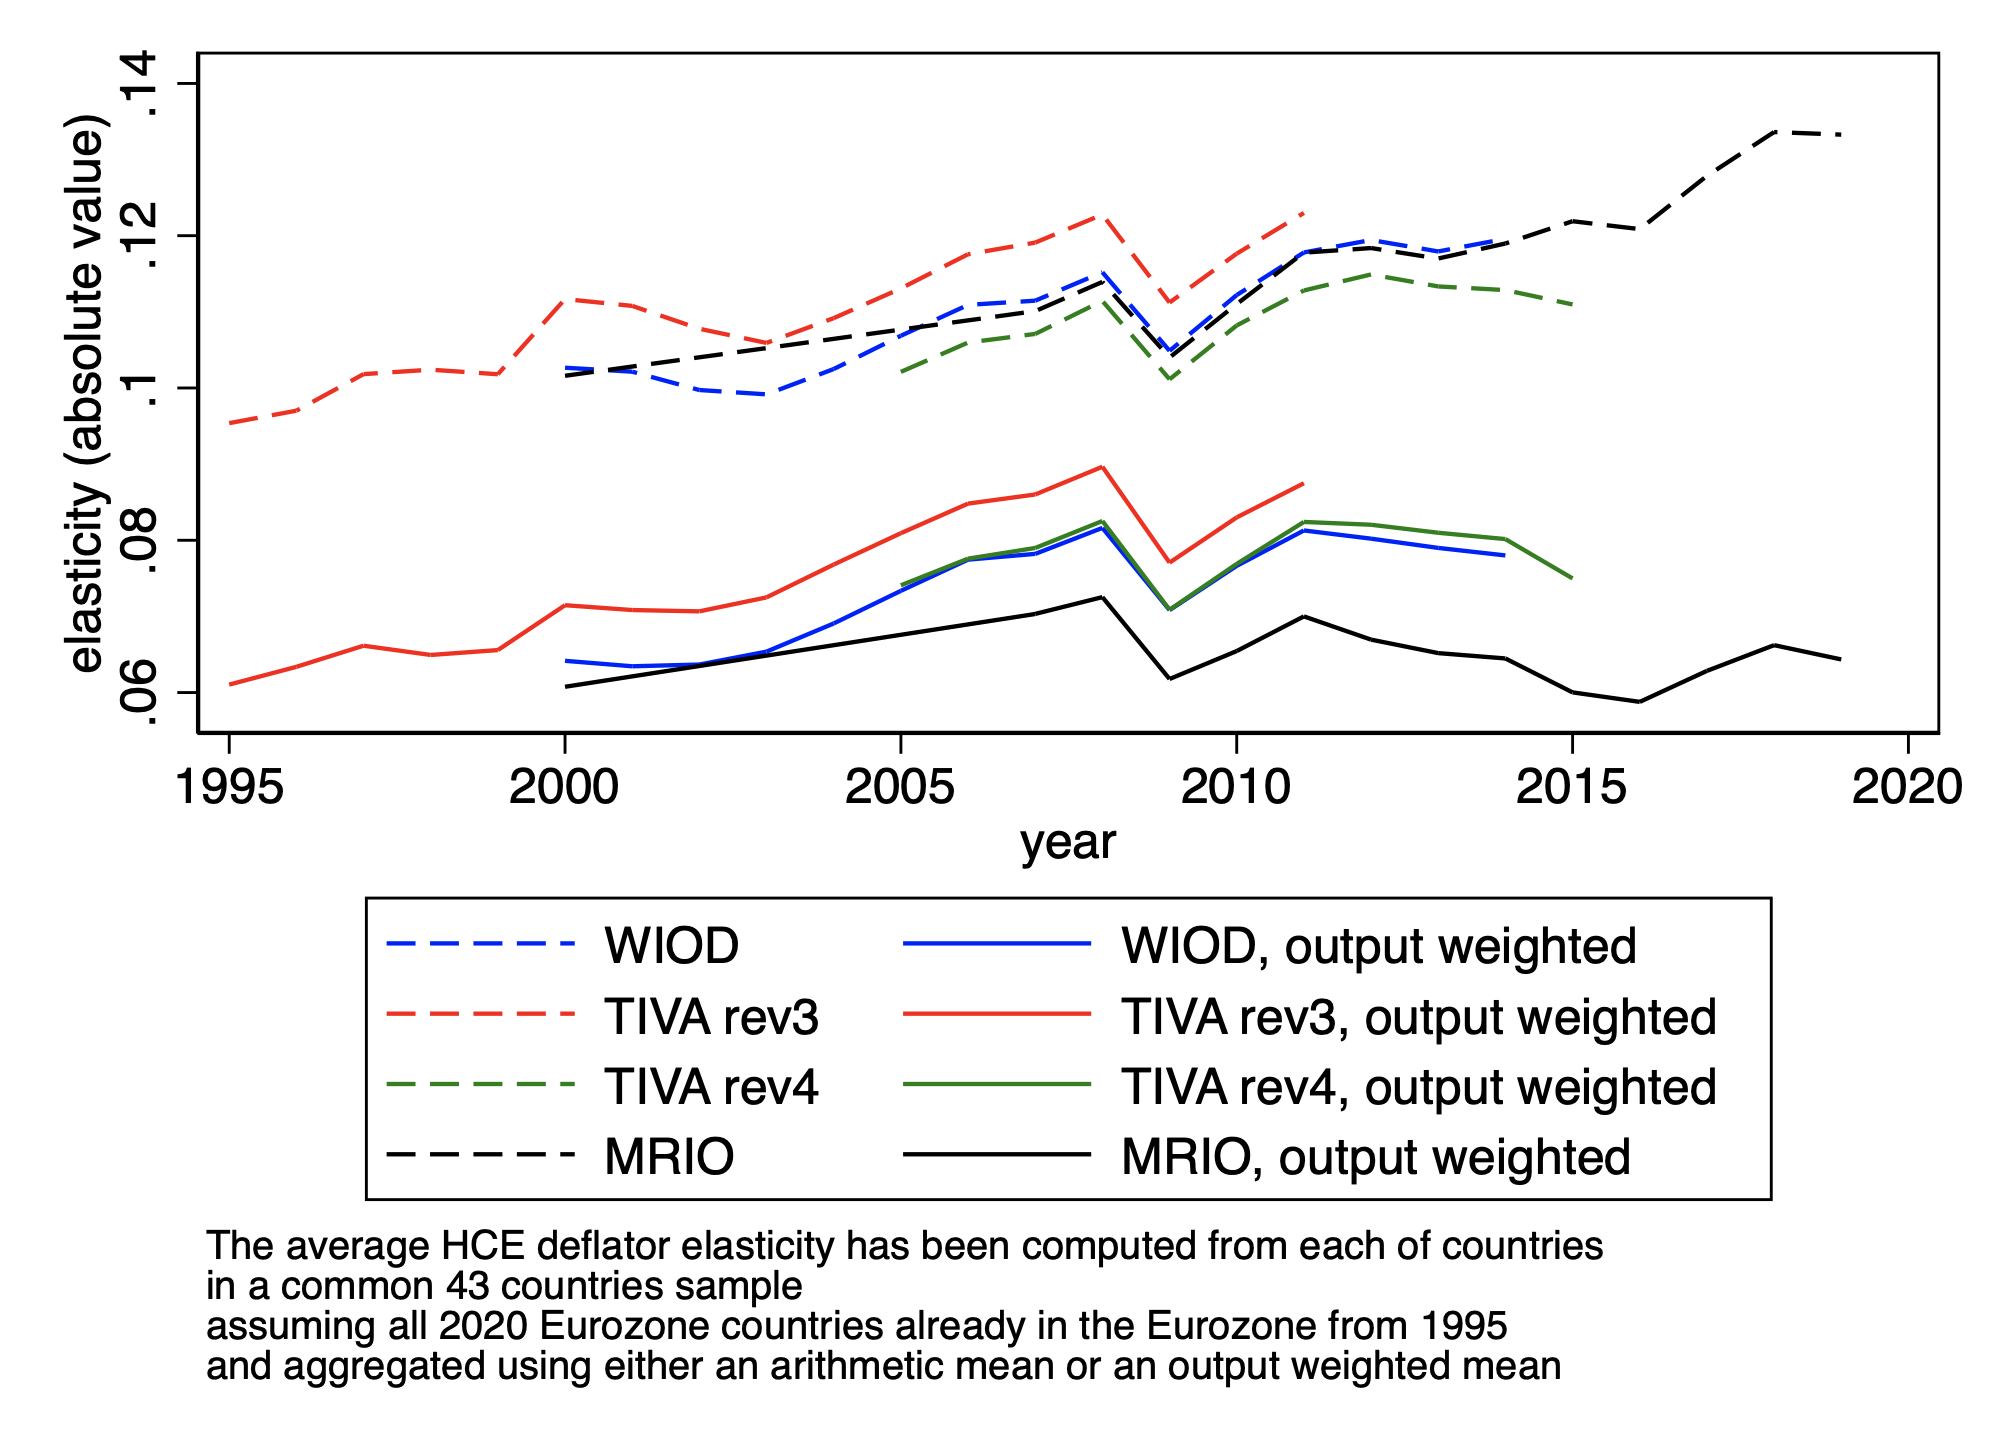
\includegraphics[width=4.5in, height=3in]{PIWIM_LONGITUDINAL.png}\\
		\floatfoot{Source: WIOD and TIVA}.
	\end{tabular}
	\label{fig:PIWIM_LONGITUDINAL}
\end{figure}



Focusing on the 2014 WIOD results, Figure \ref{fig:WIOD_HC_elasticities} shows that the absolute value of the elasticity is between .05 and .15 for most countries.
Figure \ref{fig:WIOD_HC_E1HC} shows it is closely, but not strictly, related to the share of imported goods and services in household consumption.


\begin{figure}[!h]
	\centering
	\caption{\footnotesize{\textbf{Distribution of consumer price elasticity to an exchange rate appreciation for WIOD 2014}}}
	\begin{tabular}{c}
		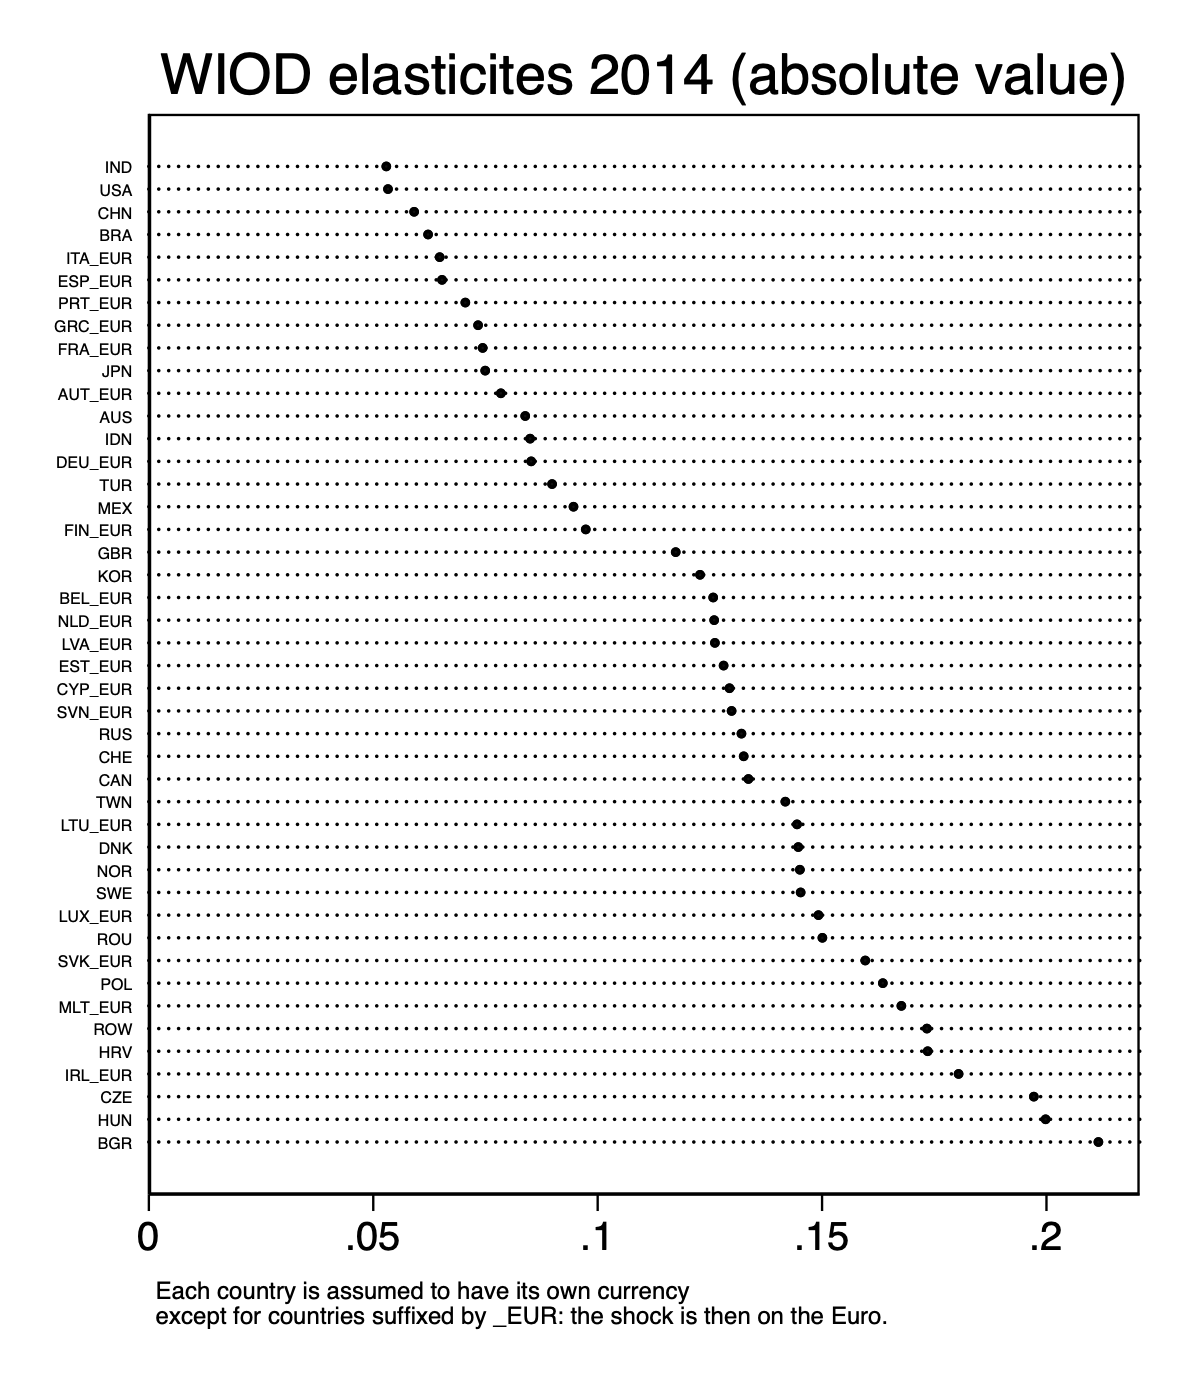
\includegraphics[width=4.5in, height=3in]
		{WIOD_HC_elasticities.png}\\
		\floatfoot{Source: WIOD}.
	\end{tabular}
	\label{fig:WIOD_HC_elasticities}
\end{figure}



\begin{figure}[!h]
	\centering
	\caption{\footnotesize{\textbf{Consumer price elasticity and share of imported consumption for WIOD 2014}}}
	\begin{tabular}{c}
		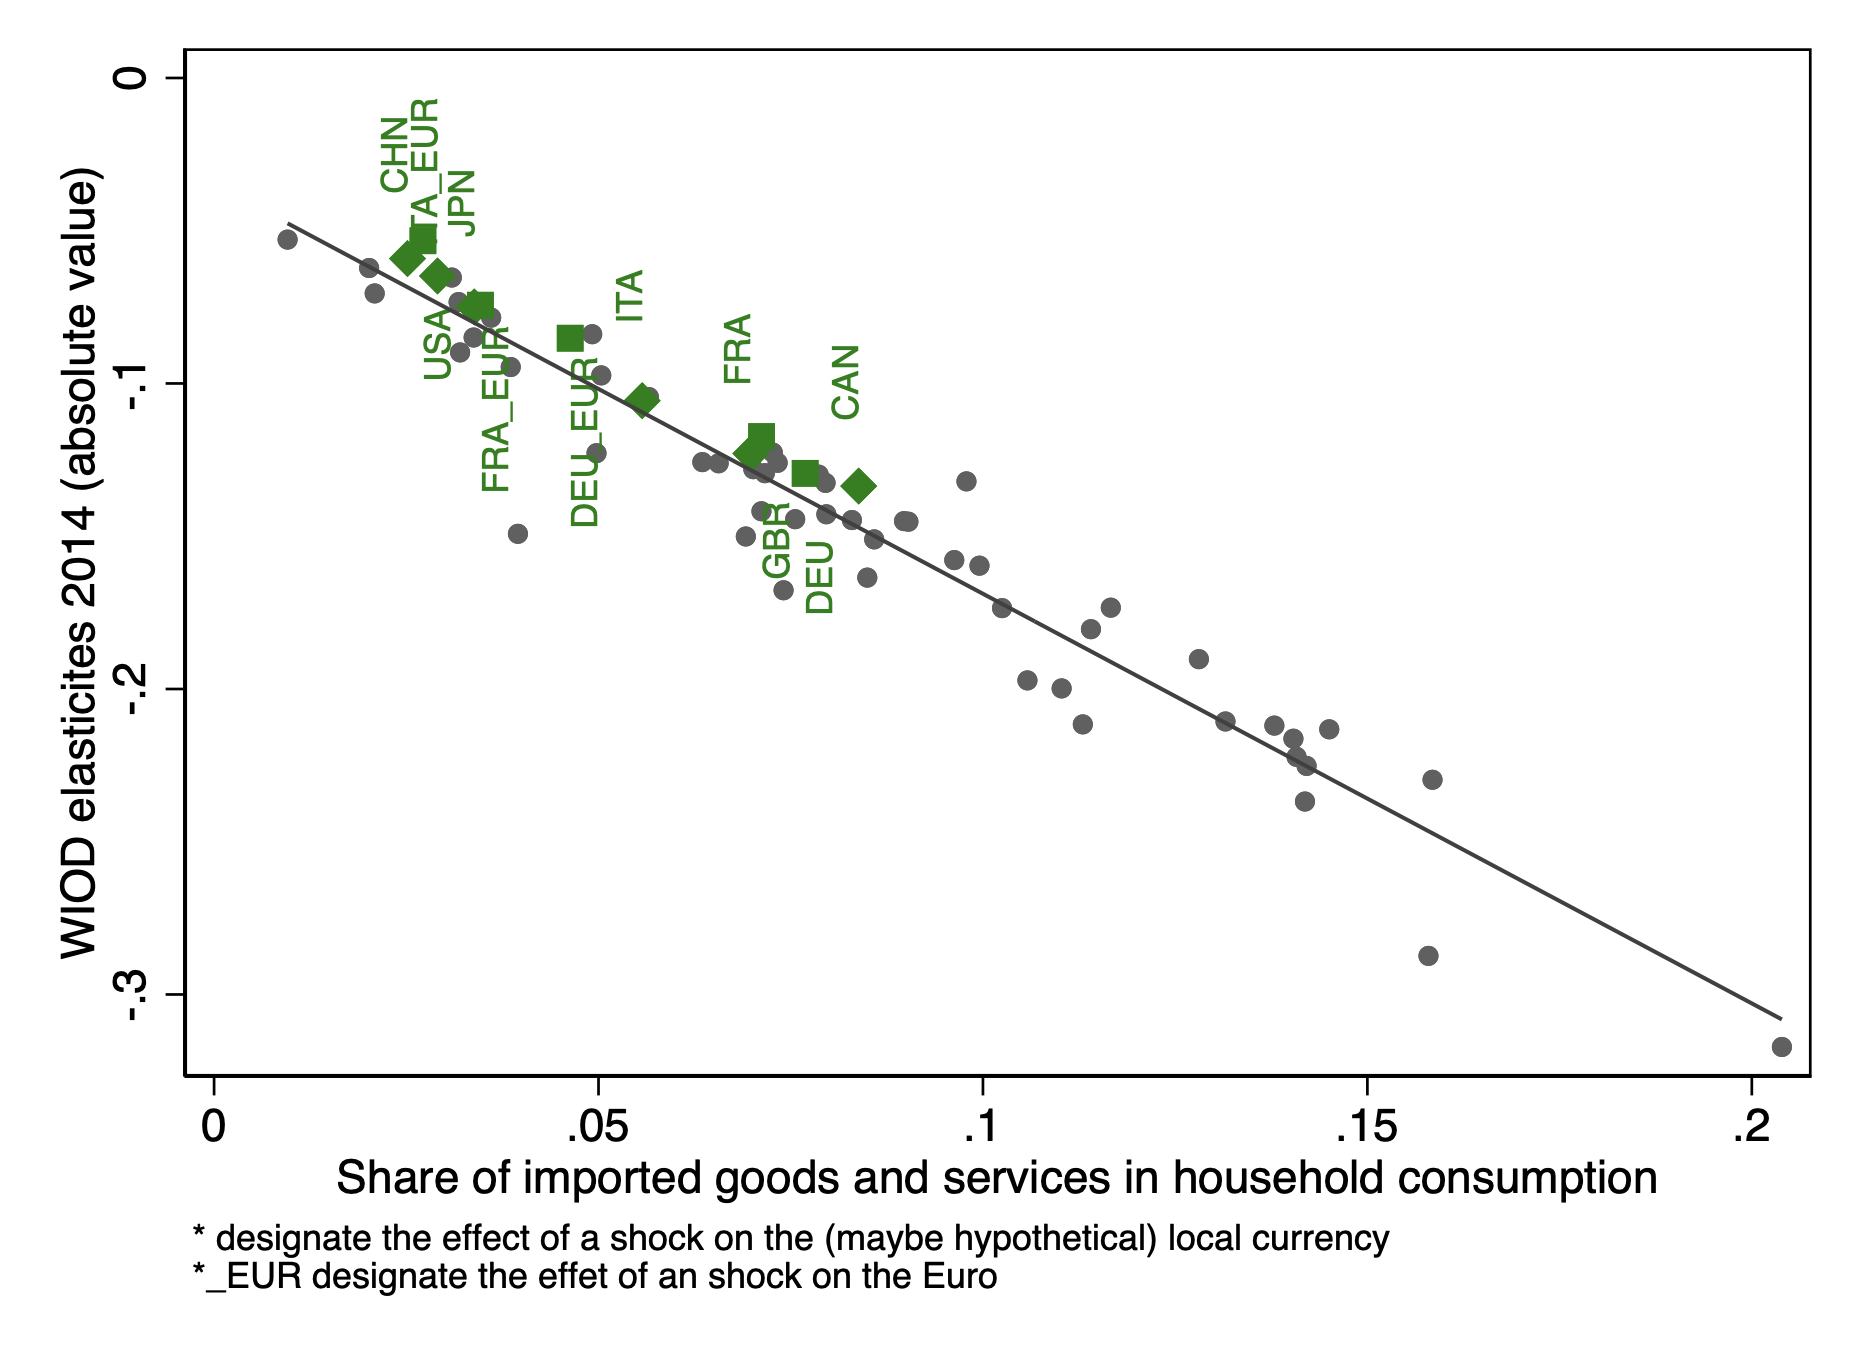
\includegraphics[width=4.5in, height=3in]
		{WIOD_HC_E1HC.png}\\
		\floatfoot{Source: WIOD}.
	\end{tabular}
	\label{fig:WIOD_HC_E1HC}
\end{figure}


\subsection{Contribution of different goods}

Looking at the contribution of different types of goods to $\overline{s_{i}}^{i,HC}$ helps understanding the mechanis at work in PIWIM. One possibility is too look at the predicted effect on domestic goods versus imported goods. We can define 
\begin{eqnarray}
\overline{s}_i^{i,HC}=\overline{s}_{i,imp}^{i,HC} + \overline{s}_{i,dom}^{i,HC} = S^i.HC^{i,dom}+ S^i.HC^{i,imp}
\label{equ:decomp_impexp}
\end{eqnarray}

Where:
\begin{equation}
\begin{array}{ccccc}
HC^i&=&HC^{i,dom} & + &  HC^{i,imp} \\ 
&=&  \left( \begin{array}{c}
	0 \\
	...\\
	\frac{{hc}_{ij}^i}{hc^i}\\
	...\\
	0
	 \end{array}
	 \right)
&+&
\left( 	\begin{array}{c} \frac{{hc}_{11}^i}{hc^i} \\	...\\0\\...\\\frac{{hc}_{IJ}^i}{hc^i}\end{array}\right) 
\end{array}
\end{equation}

For example,
\begin{equation}
\overline{s}_{i,imp}^{i,HC} = \underset{\begin{subarray}{c}j=1 \dots J   \\ k=1 \dots I \\ k \neq i \end{subarray}}{\mathop \sum}\,{{s}_{kj}^i}.\frac{{hc}_{kj}^i}{hc^i}
\label{equ:share_of_imported}
 \end{equation}


Figure \ref{fig:decomp_origine} shows that the prices of imported final consumption have the largest contribution to total effect. Although they account for a smaller share of consumption, they are more susceptible to initial shock. They are also the ones who explain the variations in the magnitude of the eslasticities between more or less open economies.

\begin{figure}[!h]
	\centering
	\caption{\footnotesize{\textbf{Contribution to consumer price elasticity of imported and domestic goods}}}
	\begin{tabular}{c}
		\includegraphics[width=4.5in, height=3in]
		{decomp_origine.png}\\
		\floatfoot{Source: WIOD, 2014}.
	\end{tabular}
	\label{fig:decomp_origine}
\end{figure}


A major part of the shock comes from lower prices for service consumption (Figure \ref{fig:decomp_sect}). This is paradoxical since, on the one hand, services are not imported a lot and, on the other hand, domestic services do not use many imported inputs. Similarly, domestic core inflation accounts for most of the shock effect for the same reason (Figure \ref{fig:decomp_sectxorigin}). These two phenomena can be explained by the significant weight in the consumption of services on the one hand and domestic services and non-energy industrial goods on the other hand.



\begin{figure}[!h]
	\centering
	\caption{\footnotesize{\textbf{Contribution to consumer price elasticity of different sectors}}}
	\begin{tabular}{c}
		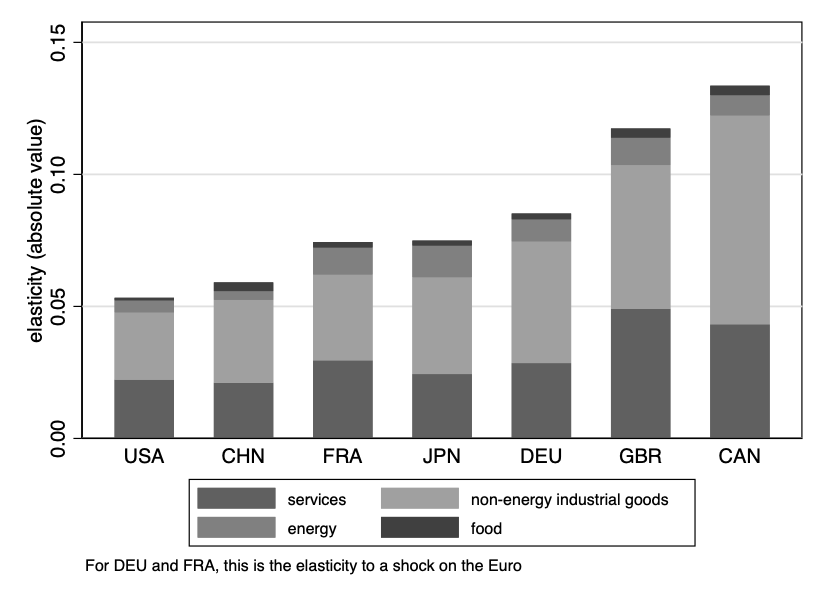
\includegraphics[width=4.5in, height=3in]
		{decomp_sect.png}\\
		\floatfoot{Source: WIOD, 2014}.
	\end{tabular}
	\label{fig:decomp_sect}
\end{figure}



\begin{figure}[!h]
	\centering
	\caption{\footnotesize{\textbf{Contribution to consumer price elasticity of different imported or domestic sectors}}}
	\begin{tabular}{c}
		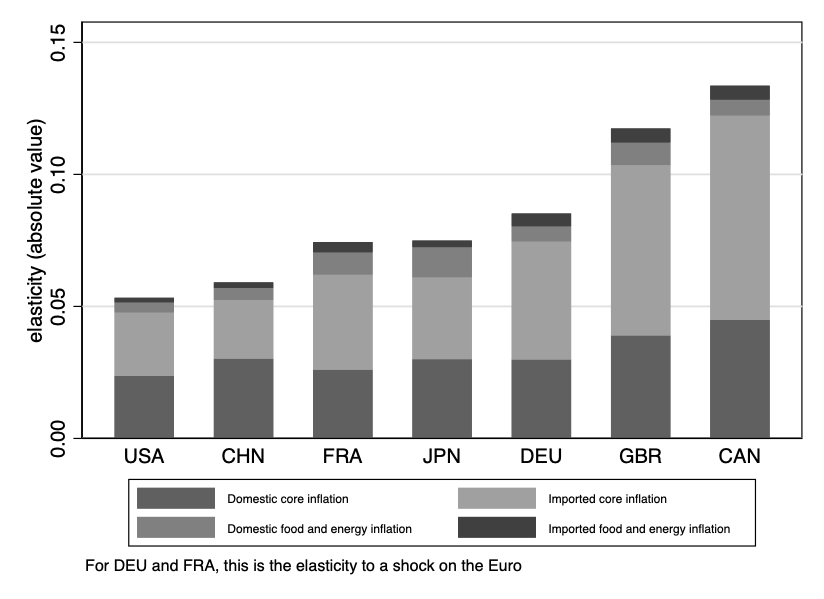
\includegraphics[width=4.5in, height=3in]
		{decomp_sectxorigin.png}\\
		\floatfoot{Source: WIOD, 2014}.
	\end{tabular}
	\label{fig:decomp_sectxorigin}
\end{figure}




%
%We can then define the contribution of imported consumption goods to an exchange rate shock as $\nicefrac{\overline{s}_{i,imp}^{i,HC}}{\overline{s}_{i}^{i,HC}} = \nicefrac{S^i.HC^{i,imp}}{S^i.HC^{i}}$. We can also define the sensitivity of imported consumption prices as $ \frac{\nicefrac{S^i.HC^{i,imp}}{S^i.HC^{i}}}{\vec{1}.HC^i,imp}$ where $\vec 1$ is a horizontal vector of ones.
%For example, if an appreciation exchange rate reduce household consumption prices by 20\%, that household consumption is 50\% imported and that imported consumption goods prices evolution cause in a reduction of household consumption prices of 15\%, then the contribution of imported consumption goods will be 0.75 (=.15/.20)and their sensitivity of 1.5 (=0.75/0.5).
%
%GD : PEUT-ÊTRE Y A-T-IL UNE MANIÈRE DE SIMPLIFIER L'EXPRESSION DE LA SENSITIVITÉ, MAIS JE NE VOIS PAS COMMENT FAIRE...
%
%Figure \ref{fig:share_impt} shows, for example, that the contribution of imported consumption is higher than 0.5 in most countries. While imported consumption has a smaller share in total consumption, this is over-compensated by the sensitivity of its prices to exchange rate shocks, as show by the comparison of \ref{fig:intensity_dom} and \ref{fig:intensity_impt}.
%
%Similar decompositions of the matrix $HC^i$ can be done to analyse the contribution of different sectors. decompose the effect between sectors. That allows the identification of the contribution of different sectors to the inflation shocks in different countries.
%Figure \ref{fig:share_sector} shows that non-energy industrial goods and services have the highest contribution. Energy is highly sensitive to exchange rate shocks (see \ref{fig:intensity_dom} and \ref{fig:intensity_impt}), but its share in consumption is too small for its contribution to the final effect to be large.
%
%
%
%\begin{figure}[p]
%\RawFloats
%\centering
%\caption{\footnotesize{\textbf{Contribution of imported final consumption to the impact of a nominal exchange rate shock (see eq. \ref{equ:share_of_imported})}}}
%\begin{tabular}{c}
%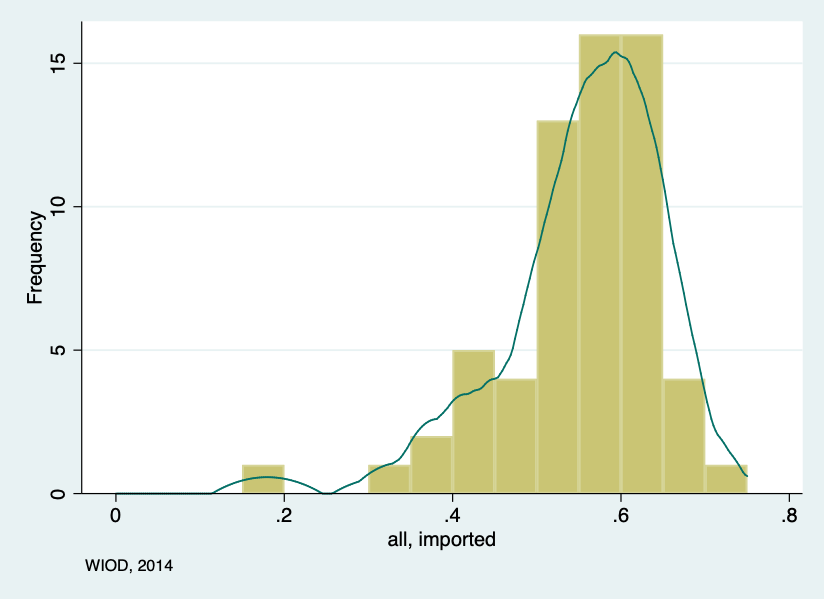
\includegraphics[width=5.0in, height=3.5in]{Share_impt_HC_WIOD_2014.png}\\
%\floatfoot{Interpretation note: the contribution of imported final consumption to the impact of a nominal exchange rate shock is between 55\% and 60\% for 16 countries}
%\end{tabular}
%\label{fig:share_impt}
%
%\caption{\footnotesize{\textbf{Contribution of sector-specific final consumption to the impact of a nominal exchange rate shock}}}
%\begin{tabular}{c}
%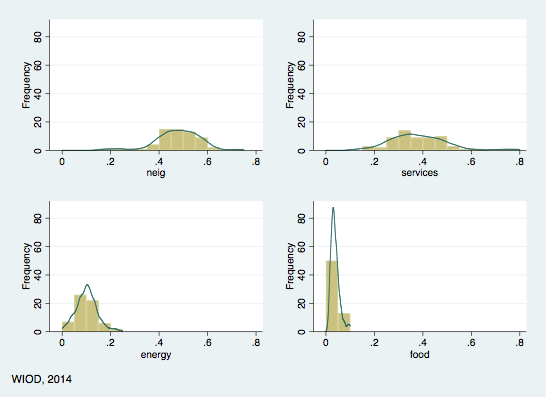
\includegraphics[width=5.0in, height=3.5in]{Share_sector_HC_WIOD_2014.png}\\
%\floatfoot{Interpretation note: the contribution of final energy consumption to the impact of a nominal exchange rate shock is lower than 15\% in most countries}
%\end{tabular}
%\label{fig:share_sector}
%\end{figure}
%
%
%
%
%\begin{figure}[p]
%\RawFloats
%\centering
%\caption{\footnotesize{\textbf{Sensitivity of different domestic sectors to an exchange rate shock}}}
%\begin{tabular}{c}
%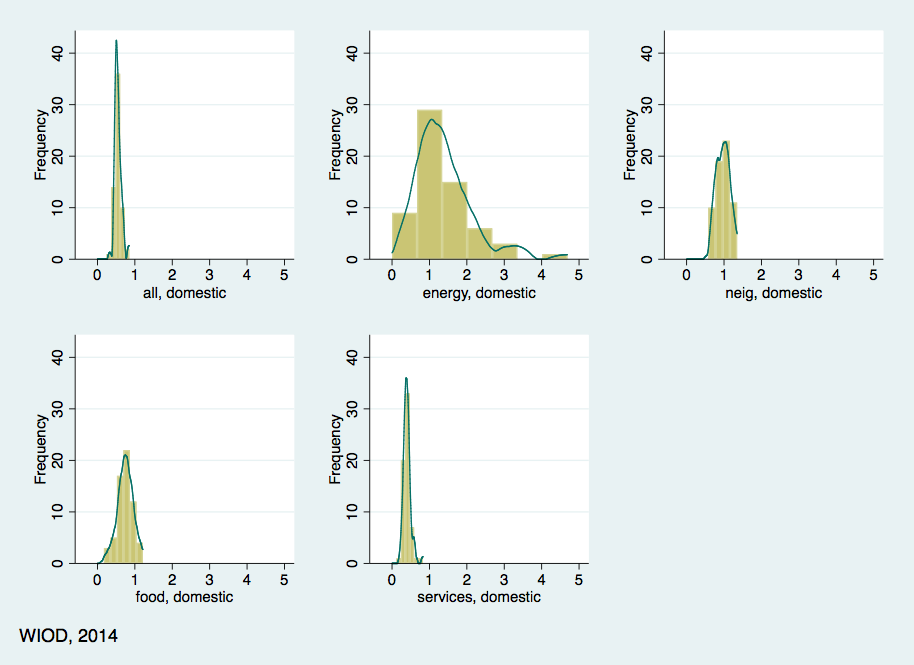
\includegraphics[width=5.0in, height=3.5in]{Int_HC_WIOD_2014_dom.png}\\
%\floatfoot{Intensity is measured as the explained share of inflation change divided by the share in final consumption}
%\end{tabular}
%\label{fig:intensity_dom}
%
%\caption{\footnotesize{\textbf{Sensitivity of imported sectors to an exchange rate shock}}}
%\begin{tabular}{c}
%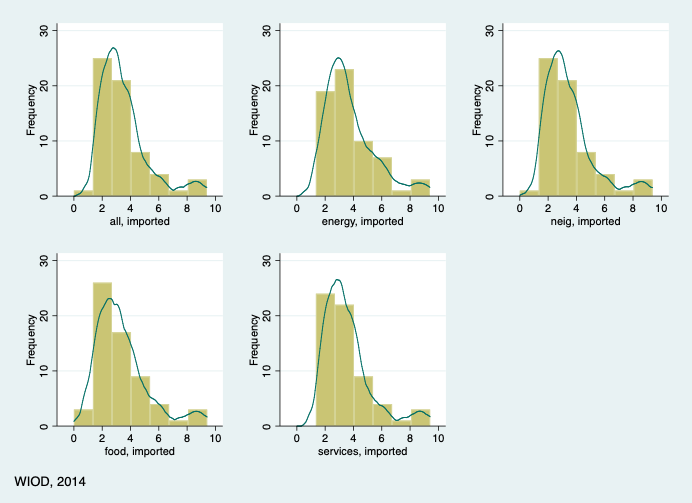
\includegraphics[width=5.0in, height=3.5in]{Int_HC_WIOD_2014_impt.png}\\
%\floatfoot{Intensity is measured as the explained share of inflation change divided by the share in final consumption}
%\end{tabular}
%\label{fig:intensity_impt}
%\end{figure}

\section{What do we gain from using world input-output matrices?}
One might wonder whether using world input-ouput matrices provided by WIOD or TIVA to compute the effect of exchange rate shocks on household consumption prices is worth the wait (the latest year covered by WIOD is 2014, and 2015 for TIVA) and the computational complexity. To answer this question, we break down $\overline{s_{i}}^{i,HC}$ into different elements classified by ease of use and computation. Let us start from equation \ref{eq:eqdomcurrency}.

\begin{equation}
\begin{array}{lccl}
	S^ i&=&C^i	&+ \left(\hat{C}^i_\$.{\cal B}+{C^i}{\tilde{{\cal B}}}\right)*{{(I-{\cal A})}^{-1}} \\
	S^i &=&\underbrace{C^i}_{\substack{\text{(E1) direct effect through} \\ \text{ imported consumption goods}}}&+ \underbrace{{C^i}{\tilde{{\cal B}}}}_{\substack{\text{(E2) effect on} \\ \text{ \emph{domestic} consumption goods} \\ \text{ through \emph{imported} inputs}}}  + \underbrace{\hat{C}^i_\$.{\cal B}}_{\substack{\text{(E3)  effect on} \\ \text{\emph{imported} consumption goods} \\ \text{through \emph{domestic} inputs}}} \\ &&+\underbrace {\left( \hat{C}^i_\$.{\cal B} + {C^i}{\tilde{{\cal B}}}\right)*{{(I-{\cal A})}^{-1}}*{\cal A}}_{\text{(E4) residual}} \\
\end{array}
\end{equation}


$C^i$ and $\hat{C}^i_\$$ have a large number of zeros. So, we have :

\begin{equation}
\begin{array}{lccl}
\overline{s}_{i}^{i,HC}&=S^i.HC^i=E1.HC^i+E2.HC^i+E3.HC^i+E4.HC^i \\
&=E1.HC^{i,imp}+E2.HC^{i,dom}+E3.HC^{i,imp}+E4.HC^i
 \end{array} 
 \end{equation}
 
When the shock corresponds to an appreciation of the domestic currency, $E1$ and $E2$ reduce country $i$'s household consumption prices and $E3$ increases country $i$'s household consumption prices. Notice that $E1$ and $E2$ are easy to compute with national input-output matrices (and do not even require inversing any matrix), whereas world input-output matrices are needed for computing $E3$ and $E4$.
 
Notice this decomposition is not the same as equation \ref{equ:decomp_impexp}. In that equation, we were interested in the contribution of different types of goods to the computed effect of the initial shock. In this equation, we are interested in the different channel through which the shock has an effect.


A first appraisal to the value-added by PIWIM is to compute the share $E1.HC^{i,imp}$, $E2.HC^{i,dom}$, $E3.HC^{i,imp}$ and $E4.HC^i$ in $\overline{s}_{i}^{i,HC}$. Figure \ref{fig:decompositionofs} provides the result. $E3.HC^{i,imp}$ is very small, $E1.HC^{i,imp}$ dominates. But, for most countries, $E4.HC^i$ represent between 10\% and 30\% of $\overline{s}_{i}^{i,HC}$.

\begin{figure}[!h]
\centering
\caption{\footnotesize{\textbf{Decomposition of $\overline{s}_{i}^{i,HC}$}}}
\begin{tabular}{c}
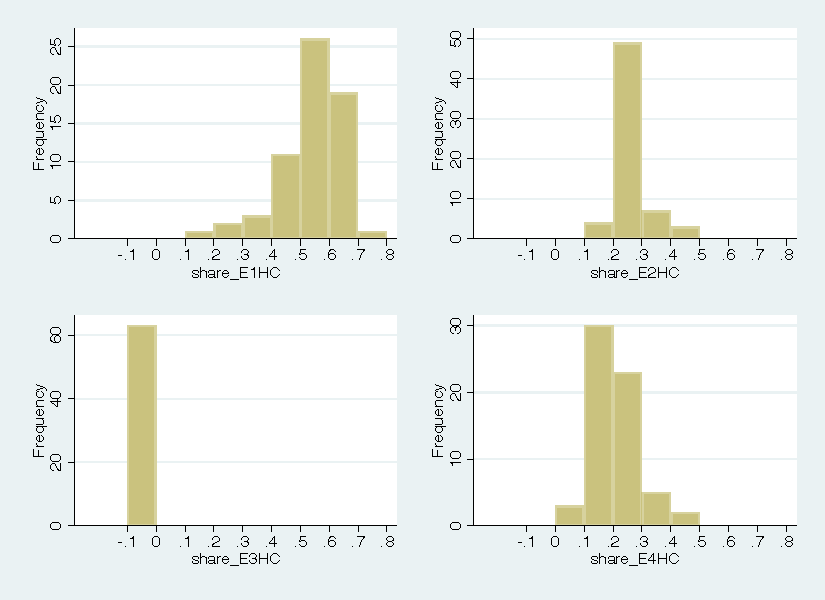
\includegraphics[width=5.0in, height=3.5in]{hist_components_WIOD}\\
\floatfoot{Source: WIOD, 2014}. \\
\end{tabular}
\label{fig:decompositionofs}
\end{figure}

Yet, the relative importance of $E4.HC^i$ might not be too much of an issue if it can be deducted from the easier-to-compute elements of $\overline{s}_{i}^{i,HC}$. This is suggested by the correlation matrix of  $E1.HC^{i,imp}$, $E2.HC^{i,dom}$, $E3.HC^{i,imp}$ and $E4.HC^i$ (see Table \ref{table:corretable_1}). 

\begin{table}[htbp]\centering \caption{Cross-correlation of $\overline{s}_{i}^{i,HC}$'s components (WIOD 2014)\label{table:corretable1}}
\begin{tabular}{l  c  c  c  c }\hline\hline
\multicolumn{1}{c}{Variables} &E1HC&E2HC&E3HC&E4HC\\ \hline
E1HC&1.00\\
E2HC&0.74&1.00\\
E3HC&-0.09&0.11&1.00\\
E4HC&0.36&0.53&0.05&1.00\\
\hline \hline 
 \end{tabular}
\end{table}


$E3.HC^{i,imp}$ does not require inversing a matrix, but it is still quite data-intensive to compute. As a result, we study wether we can deduct $\overline{s}_{i}^{i,HC}$ from $E1.HC^{i,imp}$ and $E2.HC^{i,dom}$.
Figure \ref{fig:ratiodir_WIOD} depicts the relationship between $\overline{s}_{i}^{i,HC}$ and $E1.HC^{i,imp}+E2.HC^{i,dom}$. It shows that $E1.HC^{i,imp}+E2.HC^{i,dom}$ is a pretty good predictor of $\overline{s}_{i}^{i,HC}$ (the $R^2$ is over 0.98). Excepting to some extent 2009, this relationship is constant through time (see Figure \ref{fig:evolution_b} and \ref{fig:evolution_cst}).

 \begin{equation}
\overline{s}_{i}^{i,HC}=\alpha + \beta  \left(E1.HC^{i,imp}+E2.HC^{i,dom}\right) +\varepsilon_i 
\label{eq:eq7}
 \end{equation}
 


\begin{figure}[!h]
\centering
\caption{\footnotesize{\textbf{Comparing $\overline{s}_{i}^{i,HC}$ and $E1.HC^{i,imp}+E2.HC^{i,dom}$}}}
\begin{tabular}{c}
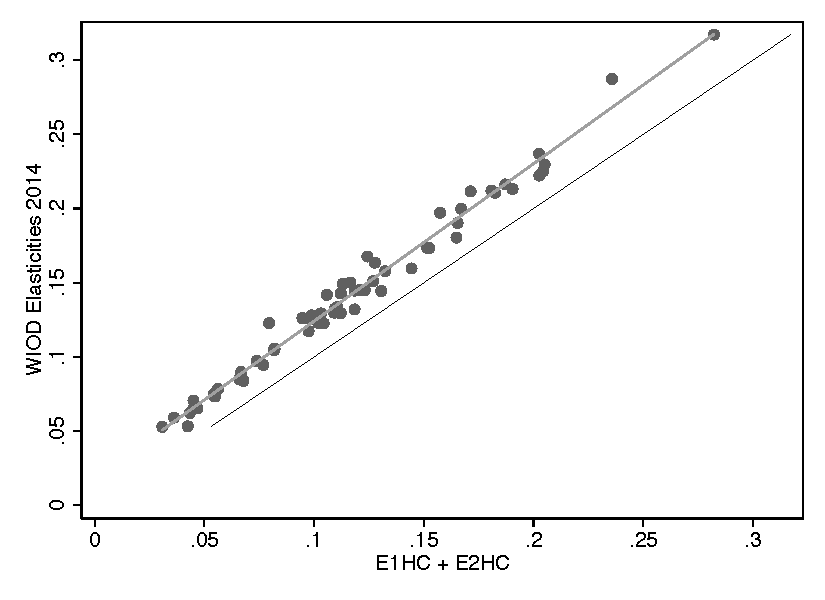
\includegraphics[width=5.0in, height=3.5in]{graph7_2014_WIOD_HC.pdf}\\
\end{tabular}
\label{fig:ratiodir_WIOD}
\end{figure}

\begin{figure}[!h]
\centering
\caption{\footnotesize{\textbf{Evolution of $\beta$ and $R2$ through time (WIOD)}}}
\begin{tabular}{c}
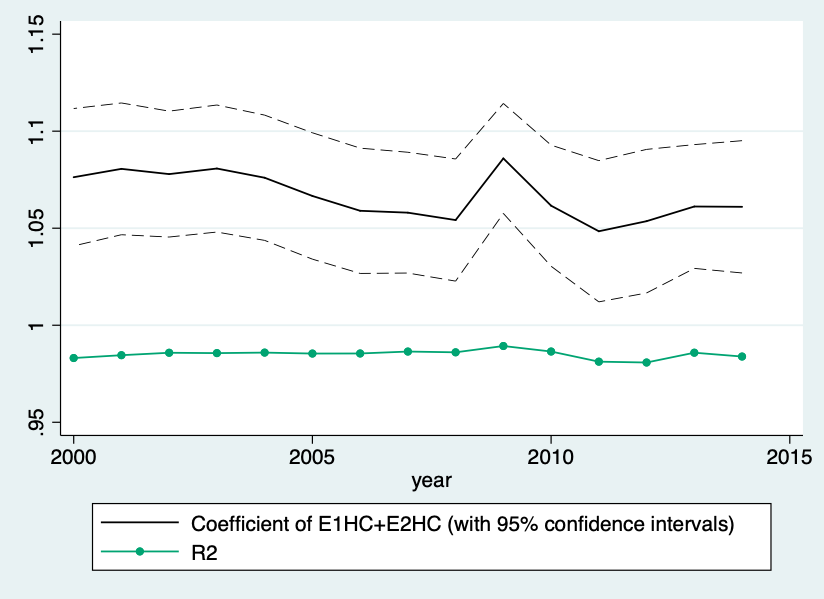
\includegraphics[width=5.0in, height=3.5in]{coef_E_WIOD_HC}\\
\end{tabular}
\label{fig:evolution_b}
\end{figure}

\begin{figure}[!h]
\centering
\caption{\footnotesize{\textbf{Evolution of $\alpha$ through time (WIOD)}}}
\begin{tabular}{c}
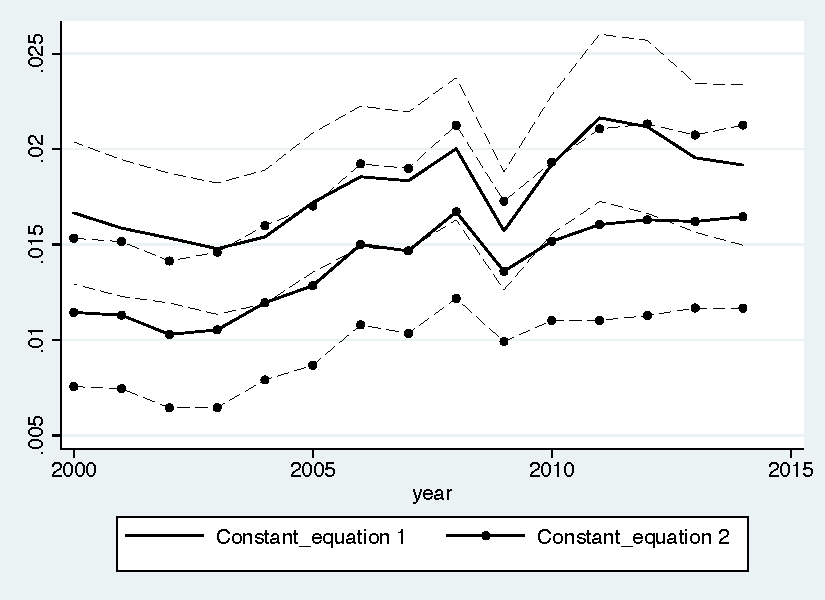
\includegraphics[width=5.0in, height=3.5in]{coef_cst_WIOD_HC}\\
\end{tabular}
\label{fig:evolution_cst}
\end{figure}


The same results mostly stand using the TiVA database (see Figures \ref{fig:ratiodir_TiVA}, \ref{fig:evolution_b_TiVA} and \ref{fig:evolution_cst_TiVA}).

\begin{figure}[!h]
\centering
\caption{\footnotesize{\textbf{Comparing $\overline{s}_{i}^{i,HC}$ and $E1.HC^{i,imp}+E2.HC^{i,dom}$ (TiVA)}}}
\begin{tabular}{c}
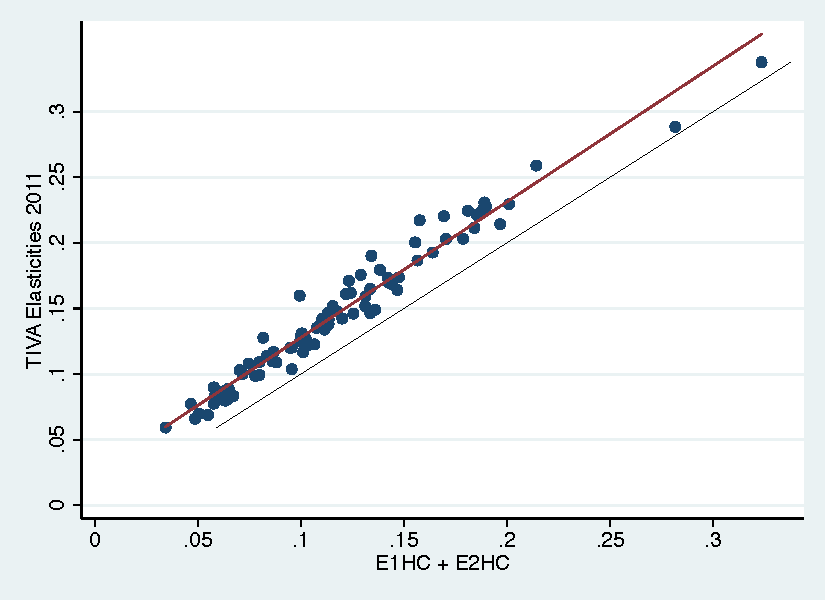
\includegraphics[width=5.0in, height=3.5in]{graph_2011_TIVA_HC}\\
\end{tabular}
\label{fig:ratiodir_TiVA}
\end{figure}

\begin{figure}[!h]
\centering
\caption{\footnotesize{\textbf{Evolution of $\beta$ and $R2$ through time (TiVA)}}}
\begin{tabular}{c}
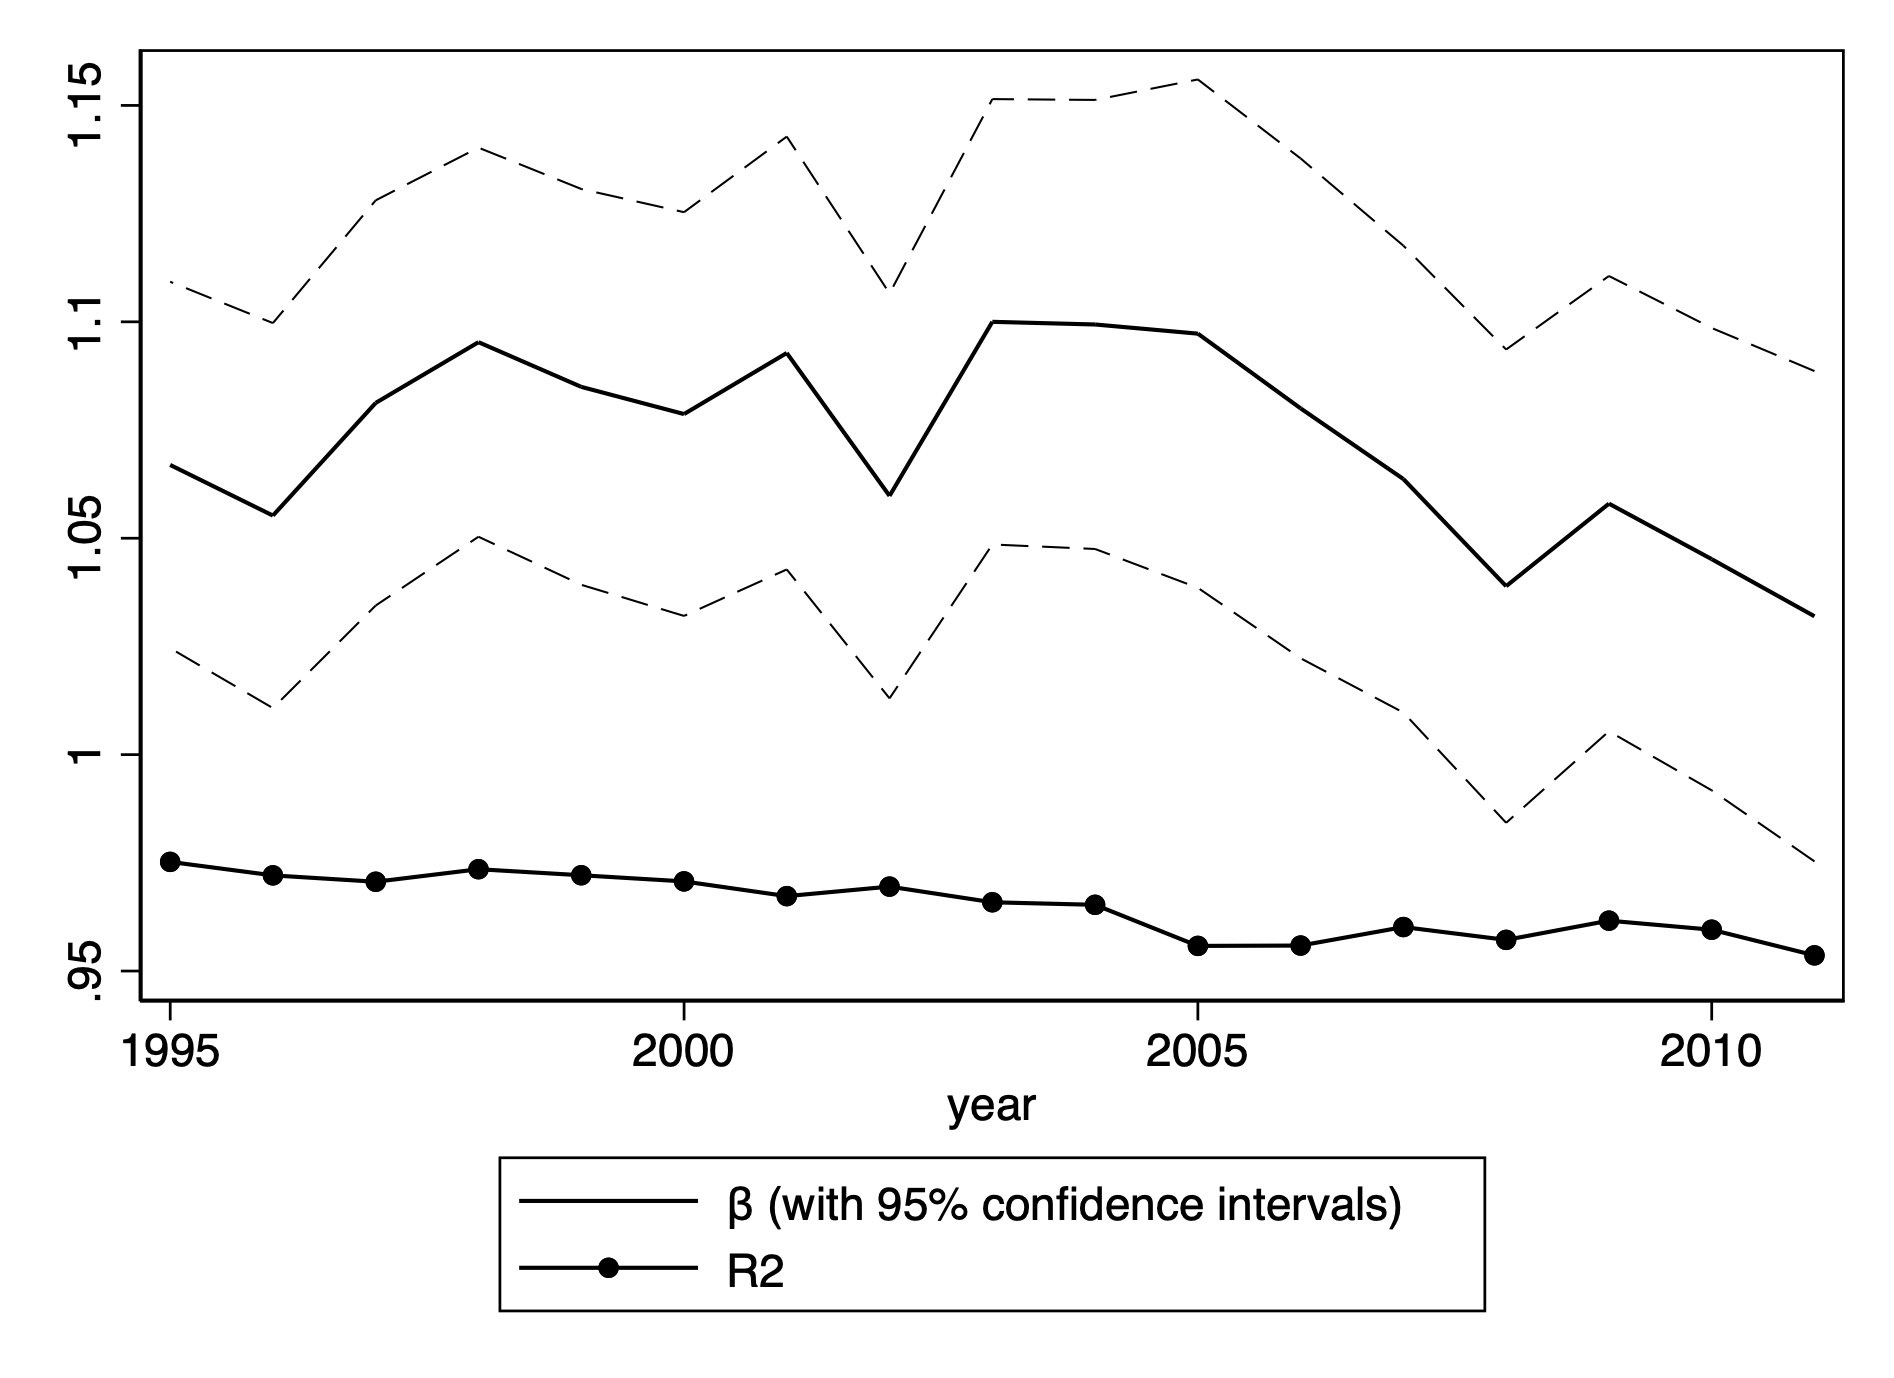
\includegraphics[width=5.0in, height=3.5in]{coef_E_TIVA_HC}\\
\end{tabular}
\label{fig:evolution_b_TiVA}
\end{figure}

\begin{figure}[!h]
\centering
\caption{\footnotesize{\textbf{Evolution of $\alpha$ through time (TiVA)}}}
\begin{tabular}{c}
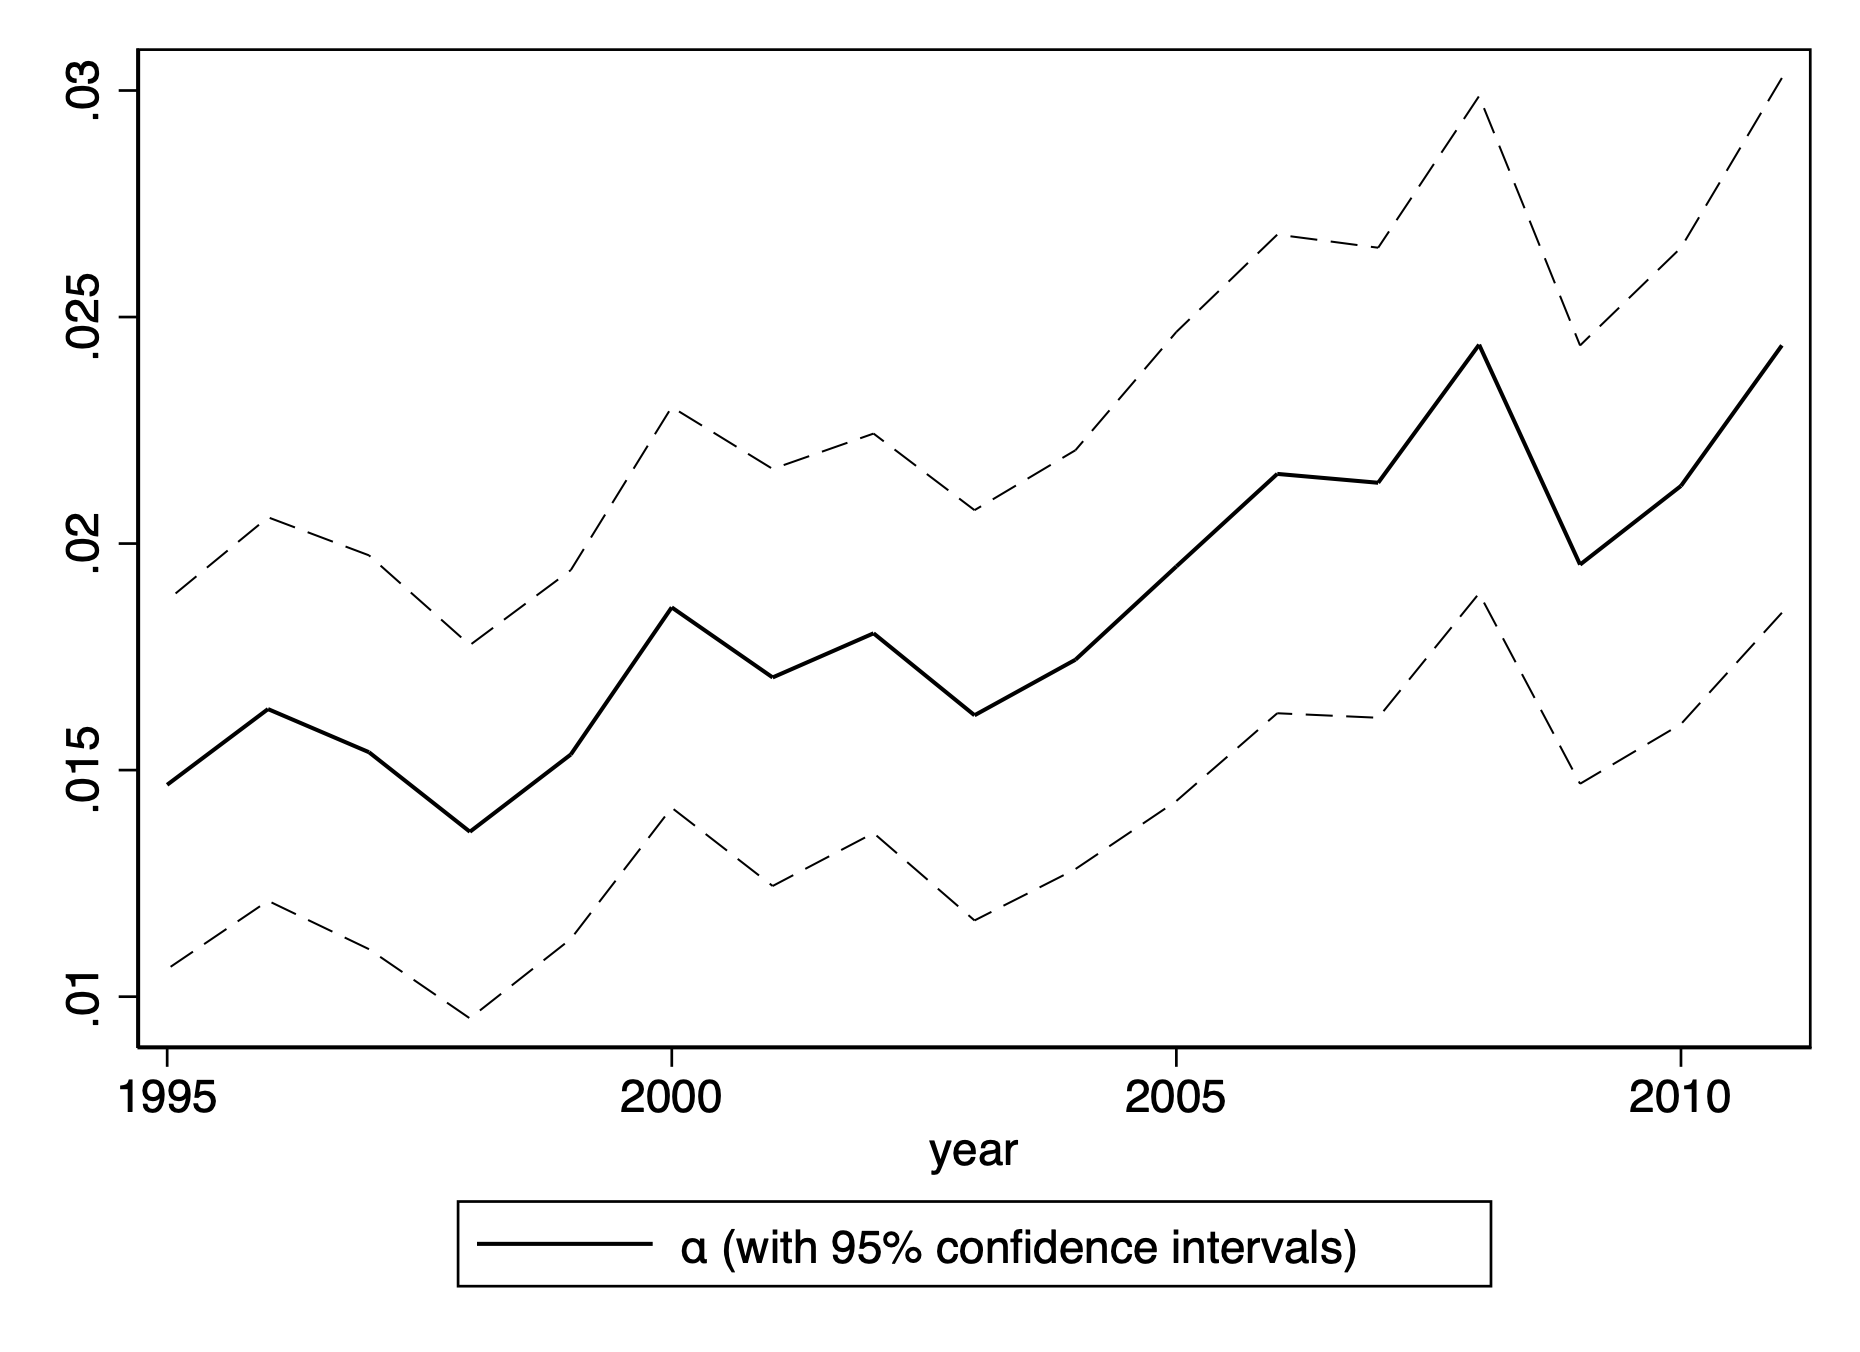
\includegraphics[width=5.0in, height=3.5in]{coef_cst_TIVA_HC}\\
\end{tabular}
\label{fig:evolution_cst_TiVA}
\end{figure}


%
%\clearpage
%
%
%\clearpage
%+++++++++++++++++++++++++++++++++++++++++++++++++++++++++
%\subsection{The intensity of import in domestic consumption}
%\label{subsec:intensity}
%
%\begin{figure}[!h]
%\centering
%\caption{\footnotesize{\textbf{The share of imported intermediate and consumer goods and services in private consumption }}}
%\begin{tabular}{c}
%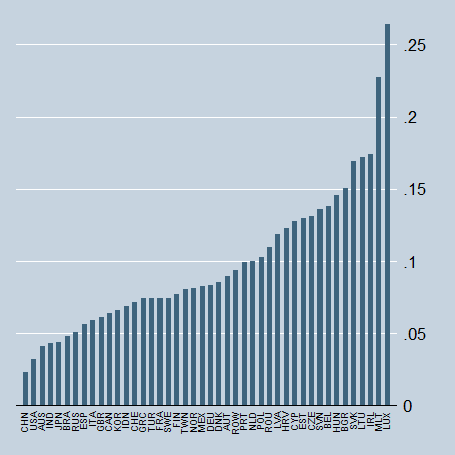
\includegraphics[width=5.0in, height=3.5in]{Graph_ratioimp_wiod_2014}\\
%\floatfoot{Source: WIOD, 2014}.
%\end{tabular}
%\label{fig:ratioimp}
%\end{figure}
%
%Differences in the import intensity across sectors and countries are crucial to our analysis on global nominal spillovers.
%In this section, we present some stylised facts about the import intensity in domestic consumption.
%Using data from the WIOD, we define the import intensity of private consumption as the share of  imported intermediate and final goods and services in total consumption. \\
%Figure \ref{fig:ratioimp} depicts the import intensity  of  household consumption in 2014.
%Not surprisingly, small countries, such as Malta, Luxembourg and Ireland, have the highest import intensity (above 15$\%$), while larger countries, such as Japan, the U.S. and Australia, display a much lower ratio of import intensity.\\
%How has the import intensity of private consumption changed over time? 
%In the Euro area, Figure \ref{fig:ratioimptemp_ze} shows that the import intensity of consumption increased in most member states over the last decade. Following the adoption of the euro, the intensity of import increased between 2000 and 2007 in all countries except the southern economies (Spain, Portugal and Greece). In the years following the Great Recession, the import intensity of consumption kept expanding in the two largest economies of the area (Germany, France), but receded in the countries stricken by the sovereign-debt crisis (Spain, Italy, Portugal and Greece).\\
%Outside of the euro area, Figure \ref{fig:ratioimptemp} shows that the import intensity of consumption has broadly expanded since 2000. 
%In all countries, except China, Croatia, Indonesia and Russia, the import intensity was higher in 2014 than it was in 2000.
%In China, it declined somewhat following the 2008-2009 crisis, reflecting global value chains shortening. In Russia, the intensity of import has been decreasing over the last two decades. 
%\begin{figure}[!h]
%\centering
%\caption{\footnotesize{\textbf{Evolution of the intensity of import in household consumption in the euro area}}}
%\begin{tabular}{c}
%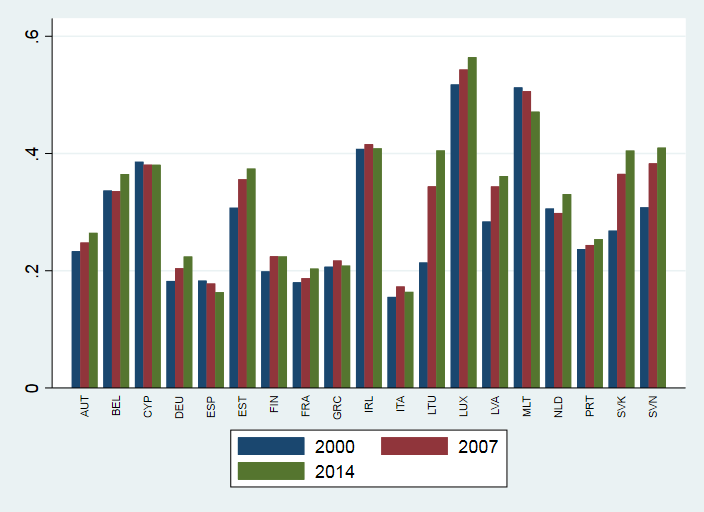
\includegraphics[width=5.0in, height=3.5in]{Graph_ratioimp_WIOD_2000_2014_ze}\\
%\floatfoot{Source: WIOD}.
%\end{tabular}
%\label{fig:ratioimptemp_ze}
%\end{figure}
%
%
%\begin{figure}[!h]
%\centering
%\caption{\footnotesize{\textbf{Evolution of the intensity of import in household consumption}}}
%\begin{tabular}{c}
%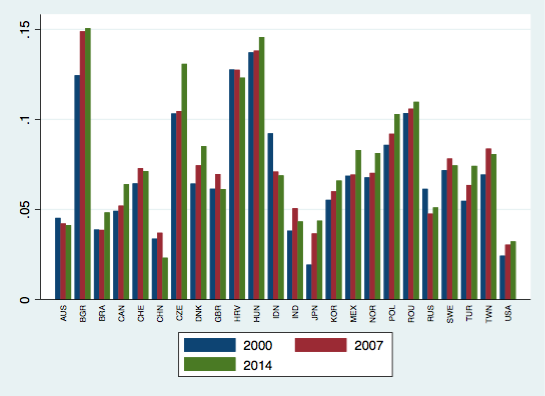
\includegraphics[width=5.0in, height=3.5in]{Graph_ratioimp_WIOD_2000_2014}\\
%\floatfoot{Source: WIOD}.
%\end{tabular}
%\label{fig:ratioimptemp}
%\end{figure}
%
%
%\subsection{The reaction of domestic consumer prices to changes in import prices}
%In this section, we evaluate how domestic consumer prices react to changes in prices of imported intermediate and final goods, the latters being caused by exchange rate fluctuations. 
%We are interested in (\textit{i}) the direct effect of global inflationary shocks, defined as the share of imported final and intermediate goods in domestic consumption (i.e. the import intensity in domestic consumption defined in Section \ref{subsec:intensity}) and (\textit{ii}) the total effect. The latter depends both on the direct effect and on the additional transmission of lower domestic input prices to other sectors of the domestic economy as well as to other countries which occurs during subsequent production cycles. 
%\paragraph{How much of domestic consumer prices' reactions to changes in import prices is explained by the direct effect?}
%
%Figure \ref{fig:ratiodir} depicts how much of the total impact of a change in import prices is explained by the import intensity of household consumption. In other words, Figure \ref{fig:ratiodir} represents the ratio of the direct effect to the total effect.
%In all countries, the direct effect accounts for more than 60$\%$ of the total impact in 2014. 
%%In five economies (India, Indonesia, Luxembourg, Mexico and Turkey), the direct effect explains more than 80$\%$ of the reaction of domestic consumer prices to changes in import prices, which suggests that these countries do not provide much intermediate goods to their partners. 
%For the whole cross-section, the coefficient of correlation between the total and the direct effect is close to unity in 2014.
%
%\begin{figure}[!h]
%\centering
%\caption{\footnotesize{\textbf{Ratio of direct to total effect of domestic consumer prices reactions to changes in import prices}}}
%\begin{tabular}{c}
%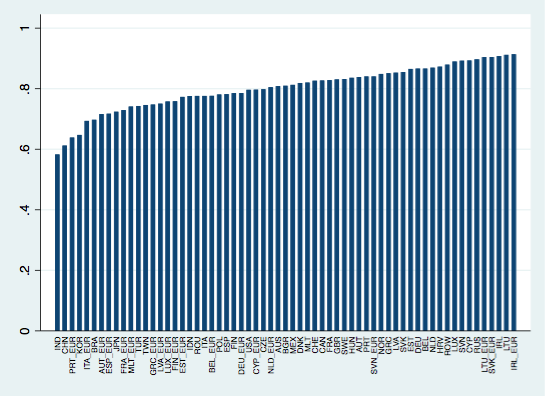
\includegraphics[width=5.0in, height=3.5in]{Graph_ratiodir_WIOD_2014}\\
%\floatfoot{Source: WIOD, 2014}.
%\end{tabular}
%\label{fig:ratiodir}
%\end{figure}
%
%
%\section{The impact of exchange rates fluctuations on the main components of consumer prices}
%\label{sec:prixconsosecteur}
%\paragraph{Differences in the intensity of import use across sectors} 
%In this section, we investigate the import intensity of consumption at the sectoral level. We run the following sectoral regressions (Equation \ref{eq:eq8}) for each sector $j$. 
%
% \begin{eqnarray}
%{S^{HC}_j}=\beta_j  I + c_j +\varepsilon
%\label{eq:eq8}
% \end{eqnarray}
% with ${S^{HC}}$ the impact of the devaluation shock on consumer prices, for each country $i$, and $I$ the vector of country-specific and sector-specific import intensity of consumption.
% 
%
%\begin{figure}[!h]
%\centering
%\caption{\footnotesize{\textbf{Consumer prices elasticity to an exchange rate shock: a sectoral analysis}}}
%\begin{tabular}{c}
%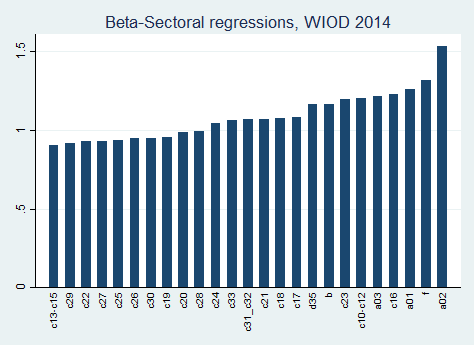
\includegraphics[width=5.0in, height=3.5in]{Graph_beta_2014_Wiod_reg_sec}\\
%\floatfoot{Source: WIOD, 2014. \\
%}
%\end{tabular}
%\label{fig:betasecteur}
%\end{figure}
%
%\begin{figure}[!h]
%\centering
%\caption{\footnotesize{\textbf{Sectoral analysis: R2}}}
%\begin{tabular}{c}
%\includegraphics[width=5.0in, height=3.5in]{Graph_r2_2014_Wiod_reg_sec}\\
%\floatfoot{Source: WIOD, 2014. \\
%}
%\end{tabular}
%\label{fig:betar2}
%\end{figure}

\section{Conclusion}
\label{sec:ccl}
Real integration through the supply chain matters for domestic price dynamics in the euro area.

\newpage
\bibliography{PapiertransmissiondeschocsenVA}
\newpage
\appendix{WIOD Sectors}
\begin{table}[!h]
 \centering
 \caption{\footnotesize{\textbf{Industries in WIOD}}}
 \footnotesize
 \begin{tabular}{ll}
  \hline \\
\textbf{A01} &{Crop and animal production, hunting and related service activities}\\
\textbf{A02} &{Forestry and logging}\\
\textbf{A03} &{Fishing and aquaculture}\\
\textbf{B} &{Mining and quarrying}\\
\textbf{C10-C12} &{Manufacture of food products, beverages and tobacco products}\\
\textbf{C13-C15} &{Manufacture of textiles, wearing apparel and leather products}\\
\textbf{C16} &{Manufacture of wood and of products of wood and cork, except furniture; articles of straw and plaiting materials}\\
\textbf{C17} &{Manufacture of paper and paper products}\\
\textbf{C18} &{Printing and reproduction of recorded media}\\
\textbf{C19} &{Manufacture of coke and refined petroleum products}\\
\textbf{C20} &{Manufacture of chemicals and chemical products}\\
\textbf{C21} &{Manufacture of basic pharmaceutical products and pharmaceutical preparations}\\
\textbf{C22} &{Manufacture of rubber and plastic products}\\
\textbf{C23} &{Manufacture of other non-metallic mineral products}\\
\textbf{C24} &{Manufacture of basic metals}\\
\textbf{C25} &{Manufacture of fabricated metal products, except machinery and equipment}\\
\textbf{C26} &{Manufacture of computer, electronic and optical products}\\
\textbf{C27} &{Manufacture of electrical equipment}\\
\textbf{C28} &{Manufacture of machinery and equipment n.e.c.}\\
\textbf{C29} &{Manufacture of motor vehicles, trailers and semi-trailers}\\
\textbf{C30} &{Manufacture of other transport equipment}\\
\textbf{C31-C32} &{Manufacture of furniture; other manufacturing}\\
\textbf{C33} &{Repair and installation of machinery and equipment}\\
\textbf{D35} &{Electricity, gas, steam and air conditioning supply}\\
\textbf{E36} &{Water collection, treatment and supply}\\
\textbf{E37-E39} &{Sewerage and other waste management services}\\
\textbf{F} &{Construction}\\
\textbf{G45} &{Wholesale and retail trade and repair of motor vehicles and motorcycles}\\
\textbf{G46} &{Wholesale trade, except of motor vehicles and motorcycles}\\
\textbf{G47} &{Retail trade, except of motor vehicles and motorcycles}\\
\textbf{H49} &{Land transport and transport via pipelines}\\
\textbf{H50} &{Water transport}\\
\textbf{H51} &{Air transport}\\
\textbf{H52} &{Warehousing and support activities for transportation}\\
\textbf{H53} &{Postal and courier activities}\\
\textbf{I} &{Accommodation and food service activities}\\
\textbf{J58} &{Publishing activities}\\
\textbf{J59-J60} &{Motion picture, video and television programme production; programming and broadcasting activities}\\
\textbf{J61} &{Telecommunications}\\
\textbf{J62-J63} &{Computer programming, consultancy; information service activities}\\
\textbf{K64} &{Financial service activities, except insurance and pension funding}\\
\textbf{K65} &{Insurance, reinsurance and pension funding, except compulsory social security}\\
\textbf{K66} &{Activities auxiliary to financial services and insurance activities}\\
\textbf{L68} &{Real estate activities}\\
\textbf{M69-M70} &{Legal and accounting activities}\\
\textbf{M71} &{Architectural and engineering activities; technical testing and analysis}\\
\textbf{M72} &{Scientific research and development}\\
\textbf{M73} &{Advertising and market research}\\
\textbf{M74-M75} &{Other professional, scientific and technical activities; veterinary activities}\\
\textbf{N} &{Administrative and support service activities}\\
\textbf{O84} &{Public administration and defence; compulsory social security}\\
\textbf{P85} &{Education}\\
\textbf{Q} &{Human health and social work activities}\\
\textbf{R-S} &{Other service activities}\\
\textbf{T} &{Activities of households as employers; producing activities of households for own use}\\
\textbf{U} &{Activities of extraterritorial organizations and bodies}\\
  	\end{tabular}
\label{tab:wiodindustries}
\end{table}

\appendix{Contrasting $S$ and $S^i$ in the two-country, one sector case}
\subsection{Evolution of VA price}
\begin{gather*}
\cal {A} = \left(\begin{matrix}a_{1,1}&a_{1,2}\\a_{2,1}&a_{2,2}\end{matrix}\right)
\\
I-\cal {A}=\left(\begin{matrix}1-a_{1,1}&-a_{1,2}\\-a_{2,1}&1-a_{2,2}\end{matrix}\right)
\\
\left(I-\cal {A}\right)^{-1}=\frac{1}{\left(1-a_{1,1}\right)\left(1-a_{2,2}\right)-a_{2,1}a_{1,2}}\left(\begin{matrix}1-a_{2,2}&a_{1,2}\\a_{2,1}&1-a_{1,1}\end{matrix}\right) =z.\left(\begin{matrix}1-a_{2,2}&a_{1,2}\\a_{2,1}&1-a_{1,1}\end{matrix}\right) \\ 
=\left(\begin{matrix}u&v\\w&x\end{matrix}\right)
\\
\text{French demand shares}=d=\left(\begin{matrix}1-f\\f\end{matrix}\right) \\
\left(I-\cal {A}\right)^{-1}d=\left(\begin{matrix}u-uf+vf\\w-wf+xf\end{matrix}\right)
\end{gather*}

Donc, en cas de choc $c$ pour le prix de la va dans le pays étranger (en monnaie française), on peut écrire un vecteur de choc : $C=\left(0,c\right)$.  les prix varient tout d'abord de  $C\cal {A}$, puis $C\cal {A}^2$, etc. Donc le vecteur de choc $S$ (en monnaie française) est : 


\begin{equation*}
S=C+C\cal {A}+C\cal {A}^2...=C(I-\cal {A})^{-1}=\left(\begin{matrix}cw  &   cx\end{matrix}\right)
\end{equation*}

To measure the effect on French consumption prices, we do a weighted sum of these effects.

\begin{equation}
\bar{s}=c.\left[\left(1-f\right)w+xf\right]=c.\frac{\left(1-f\right)a_{2,1}+f\left(1-a_{1,1}\right)}{\left(1-a_{1,1}\right)\left(1-a_{2,2}\right)-a_{2,1}a_{1,2}}
\end{equation}

If each nation's production only uses national inputs, we have a plausible :
\begin{equation*}
\bar{s}=c.\frac{f}{1-a_{2,2}}
\end{equation*}

\subsection{Exchange rate shock}

Using the notations in the paper...

\begin{gather*}
C=\left(0,\frac{-c_\$}{1+c_\$}\right)=\left(0,-c\right)
\\
C_\$=\left(c_\$,0\right)
\\
\tilde{C}_\$=\left(0,-c_\$\right)
\\
\hat{C}_\$=\left(\frac{c_\$}{1+c_\$},0\right)=\left(c,0\right)
\\
\cal B = \left(\begin{matrix}0&a_{1,2}\\0&0\end{matrix}\right)
\\
\tilde{\cal B} = \left(\begin{matrix}0&0\\a_{2,1}&0\end{matrix}\right)
\end{gather*}

Hence

\begin{gather*}
S =\left(0,c\right)+\left[\left(0,-c.a_{1,2}\right)+\left(c.a_{2,1},0\right)\right]*\left(\begin{matrix}u&v\\w&x\end{matrix}\right)
\\
=\left(0,c\right)+\left(c.a_{2,1},-c.a_{1,2}\right)*\left(\begin{matrix}u&v\\w&x\end{matrix}\right)
\\
=\left(0,c\right)+\left(u.c.a_{2,1}-w.c.a_{1,2},v.c.a_{2,1}-x.c.a_{1,2}\right)
\\
=\left(u.c.a_{2,1}-w.c.a_{1,2},c+v.c.a_{2,1}-x.c.a_{1,2}\right)
\end{gather*}
and
\begin{gather*}
\bar{s}=\left(u.c.a_{2,1}-w.c.a_{1,2},c+v.c.a_{2,1}-x.c.a_{1,2}\right).\left(\begin{matrix}1-f\\f\end{matrix}\right)
\\
\bar{s}=c\left[f\left(1+v.a_{2,1}-x.a_{1,2}\right)+\left(1-f\right)\left(u.a_{2,1}-w.a_{1,2}\right)\right]
\end{gather*}


If each nation's production only uses national inputs, we have a plausible

\begin{gather*}
\bar{s}=c.f
\end{gather*}

This seems to confirm that the exchange rate shock is not the same as the VA price shock.



\end{document}